\secnumbersection{VALIDACIÓN DE LA SOLUCIÓN}
Este capítulo presenta la validación experimental de la propuesta. Se describen primero los casos de prueba empleados, los métodos de comparación y el protocolo de evaluación, para luego reportar los resultados obtenidos, los límites identificados del método y su capacidad de generalización. La totalidad de las implementaciones utilizadas en esta validación, incluyendo el entorno de simulación, el agente y los métodos de comparación, se encuentra disponible públicamente en el repositorio del proyecto~\cite{RepositorioPVRP}.

%=============================================================%
\subsection{Instancias de evaluación} \label{sec:Instanciasdeevaluacion}
%=============================================================%
Para asegurar una evaluación completa que cubra distintos niveles de dificultad, se seleccionó un conjunto representativo de instancias del repositorio global~\cite{NEO2013}. Antes de detallar la métrica, conviene recordar la notación empleada para caracterizar cada instancia: $N$ es el número de clientes, $T$ el horizonte de planificación en días, $|K|$ el número de vehículos disponibles por día, $Q$ la capacidad de cada vehículo, y la \textit{saturación} el porcentaje de utilización de la capacidad total de la flota respecto a la demanda de la instancia. La Tabla~\ref{table:MetodoEvaluacion} presenta las características de estos problemas, agrupados en tres familias estructurales.

\begin{table}[H]
    \centering
    \caption{\label{table:MetodoEvaluacion} Instancias consideradas para la evaluación experimental.}
    \caption*{Fuente: Elaboración propia.}
    \renewcommand{\arraystretch}{1.12}
    \setlength{\tabcolsep}{10pt}
    \begin{tabular}{@{}ccccccc@{}}
        \toprule
        \textbf{Familia} & \textbf{Instancia} & $N$ & $T$ & $|K|$ & $Q$ & \textbf{Saturación} \\
        \midrule
        \multirow{3}{*}{A}
        & $p01$ & $50$  & $2$ & $3$ & $160$ & $81\%$ \\
        & $p04$ & $75$  & $2$ & $5$ & $140$ & $97\%$ \\
        & $p07$ & $100$ & $2$ & $4$ & $200$ & $91\%$ \\
        \midrule
        \multirow{3}{*}{B}
        & $p02$ & $50$  & $5$ & $3$ & $160$ & $86\%$ \\
        & $p05$ & $75$  & $5$ & $6$ & $140$ & $82\%$ \\
        & $p08$ & $100$ & $5$ & $5$ & $200$ & $79\%$ \\
        \midrule
        \multirow{3}{*}{C}
        & $p03$ & $50$  & $5$  & $1$ & $160$ & $97\%$ \\
        & $p06$ & $75$  & $10$ & $1$ & $140$ & $97\%$ \\
        & $p09$ & $100$ & $8$  & $1$ & $200$ & $91\%$ \\
        \bottomrule
    \end{tabular}
\end{table}

Como se observa en la Tabla~\ref{table:MetodoEvaluacion}, las instancias varían en tamaño ($50$, $75$ y $100$ clientes) y se dividen según su complejidad intrínseca. La familia A presenta un horizonte corto con varios vehículos, pero sin multi-frecuencia. La familia B introduce el escenario más difícil, con un horizonte medio y el requerimiento de multi-frecuencia, entendida como la necesidad de que un mismo cliente sea visitado más de una vez a lo largo del horizonte de planificación, siguiendo un patrón de días válido. La familia C plantea un horizonte mucho más largo donde un solo vehículo debe encargarse de todo el ruteo.

Clasificar las instancias de esta forma, como se resume en la Tabla~\ref{table:Familias}, resulta clave para el análisis, pues permite aislar las variables y entender qué es lo que realmente le cuesta al modelo: si la dificultad proviene de una red muy grande (escala de clientes) o de las restricciones de tiempo y frecuencia de visita.

\begin{table}[H]
    \centering
    \caption{\label{table:Familias} Familias de instancias utilizadas en la evaluación.}
    \caption*{Fuente: Elaboración propia.}
    \renewcommand{\arraystretch}{1.18}
    \setlength{\tabcolsep}{9pt}
    \begin{tabular}{
        @{}
        >{\raggedright\arraybackslash}m{3.1cm}
        >{\raggedright\arraybackslash}m{5.2cm}
        >{\centering\arraybackslash}m{1.1cm}
        >{\centering\arraybackslash}m{1.1cm}
        >{\centering\arraybackslash}m{1.1cm}
        @{}
    }
        \toprule
        \textbf{Familia}
        & \textbf{Características}
        & \multicolumn{3}{c}{\textbf{Instancias}} \\
        \cmidrule(lr){3-5}
        & & \textbf{50} & \textbf{75} & \textbf{100} \\
        \midrule
        A - Simple
        & \begin{tabular}[c]{@{}l@{}}
            Horizonte corto \\
            Múltiples vehículos \\
            Sin multi-frecuencia
          \end{tabular}
        & $p01$ & $p04$ & $p07$ \\
        \addlinespace[4pt]
        B - Difícil
        & \begin{tabular}[c]{@{}l@{}}
            Horizonte medio \\
            Múltiples vehículos \\
            Multi-frecuencia
          \end{tabular}
        & $p02$ & $p05$ & $p08$ \\
        \addlinespace[4pt]
        C - Largo
        & \begin{tabular}[c]{@{}l@{}}
            Horizonte extendido \\
            Un único vehículo \\
            Sin multi-frecuencia
          \end{tabular}
        & $p03$ & $p06$ & $p09$ \\
        \bottomrule
    \end{tabular}
\end{table}

Es importante destacar que esta selección no es arbitraria, sino que responde a un diseño factorial completo de dos factores: la familia estructural (A, B, C) y la escala de clientes ($50$, $75$, $100$). El cruce de ambos factores produce las nueve celdas que se evalúan en este estudio, tal como resume la Tabla~\ref{table:CoberturaFactorial}. Este diseño permite aislar el efecto de cada factor sobre el desempeño del método: comparando dentro de una misma familia se observa el impacto puro de la escala, mientras que comparando a igual escala entre familias se observa el impacto puro de la estructura del problema.

\begin{table}[H]
    \centering
    \caption{\label{table:CoberturaFactorial} Diseño factorial $3 \times 3$ de la evaluación: familia estructural por escala de clientes.}
    \caption*{Fuente: Elaboración propia.}
    \renewcommand{\arraystretch}{1.25}
    \setlength{\tabcolsep}{12pt}
    \begin{tabular}{@{}cccc@{}}
        \toprule
        & \textbf{50 clientes} & \textbf{75 clientes} & \textbf{100 clientes} \\
        \midrule
        \textbf{Familia A} & $p01$ & $p04$ & $p07$ \\
        \textbf{Familia B} & $p02$ & $p05^{*}$ & $p08^{*}$ \\
        \textbf{Familia C} & $p03$ & $p06$ & $p09$ \\
        \bottomrule
    \end{tabular}
\end{table}

Respecto a la cobertura del estudio, cabe precisar su alcance. Las instancias del conjunto NEO empleadas constituyen un estándar consolidado para el PVRP clásico, y el diseño factorial descrito cubre sistemáticamente la variación en escala y estructura que caracteriza a este problema. Las celdas marcadas con un asterisco ($p05$ y $p08$, familia B en escalas de $75$ y $100$ clientes) se excluyen del entrenamiento del agente sobre la base del resultado sistemático de infactibilidad observado en $p02$ (familia B, $50$ clientes), documentado en la Sección~\ref{sec:limites}; los métodos de comparación sí se ejecutan sobre ellas. Por otra parte, variantes más ricas del problema, como aquellas que incorporan ventanas de tiempo, demandas estocásticas o múltiples depósitos, quedan fuera del alcance de esta memoria y se plantean como líneas de trabajo futuras en el Capítulo 5. 

%\eli{¿no hay más instancias PVRP en la literatura?} \javi{Profe, respondo acá: expliqué que las 9 instancias son un diseño factorial 3x3 (familia x escala), no una selección arbitraria, y agregué la Tabla~\ref{table:CoberturaFactorial} para mostrarlo. También aclaré el alcance: p05 y p08 se excluyen por el límite de familia B, y las variantes con ventanas de tiempo o demanda estocástica quedan como trabajo futuro.}

%=============================================================%
\subsection{Métodos de comparación} \label{sec:Metodosdecomparacion}
%=============================================================%
Para evaluar objetivamente la calidad de las soluciones generadas por el agente, se implementaron dos métodos de referencia que representan distintos niveles de complejidad. Ambos actúan como líneas base para contrastar tanto la eficiencia computacional como el desempeño en la optimización de la política aprendida.

El primer método es una \textbf{Heurística Constructiva Voraz (Greedy)}, una implementación propia basada en la clásica estrategia del vecino más cercano, adaptada al horizonte periódico. Primero asigna un patrón de días a cada cliente; luego, para cada jornada, construye las rutas eligiendo siempre al cliente disponible físicamente más cercano, hasta que el vehículo agota su capacidad. Al ser un enfoque \enquote{miope}, solo busca la mejor opción inmediata sin considerar su impacto sobre el resto de la planificación. Es una línea base sencilla y \textbf{determinista}, cuya principal ventaja es que calcula las soluciones casi al instante.

El segundo método es la \textbf{Metaheurística de Búsqueda de Entorno Variable (VNS)}, reconocida en la literatura como uno de los enfoques más efectivos para resolver el PVRP~\cite{HEMMELMAYR2009791} y cuyo funcionamiento se detalló en la Sección~\ref{sec:Aplicaciones}. Se implementó siguiendo los lineamientos metodológicos de Hemmelmayr et al.~\cite{HEMMELMAYR2009791}, adaptándolo a la representación de este trabajo, y se configuró con $100$ iteraciones para todas las instancias. \eli{Indicar en qué lenguaje se implementó}. \eli{El VNS está descrito de manera muy general. Indicar representación, inicialización, movimientos, perturbación y parámetros relevantes}. Por su capacidad de refinamiento iterativo, se escoge como el rival principal contra el cual se contrasta el desempeño del agente.

%\eli{¿Alguno es de la literatura? ¿Hay resultados en la literatura para comparación?} \eli{¿de la literatura?} \eli{Es determinista, ¿no?} \eli{¿Se implementa la propuesta de Hemmelmayr? ¿Es su código? Está explicada en el estado del arte. Indicar.}

%\javi{Respondo todos acá profe: (1) VNS viene de la literatura (Hemmelmayr et al. 2009), Greedy es implementación propia estándar del vecino más cercano. (2) El VNS es implementación propia siguiendo el esquema del paper, no su código original. (3) Sí, Greedy es determinista. (4) Quité la re-explicación del mecanismo de VNS porque ya está en el estado del arte (Sección 2.2.3), y desde acá remito. Configuré VNS con 100 iteraciones.}

%=============================================================%
\subsection{Métodos de evaluación} \label{sec:Metodosdeevaluacion}
%=============================================================%
Para validar la propuesta, la etapa de experimentación se organiza en torno a tres grandes ejes, que definen las dimensiones bajo las cuales se juzga el desempeño del agente.

\begin{itemize}
    \item \textbf{Calidad:} Mide la diferencia porcentual o \emph{gap} entre el costo de las rutas que genera el agente y el mejor resultado conocido en la literatura (\emph{Best Known Solution}, BKS). Permite determinar qué tan buenas son las soluciones obtenidas en comparación con los métodos de referencia y los resultados óptimos.

    \item \textbf{Robustez:} Dado que el algoritmo PPO incorpora un componente estocástico, su desempeño depende de la semilla aleatoria inicial. Por ello es necesario comprobar que los buenos resultados no sean producto del azar. Para esto, cada instancia se entrena con cinco semillas distintas, lo que permite medir el promedio y la desviación estándar del \emph{gap}, además de la proporción de corridas que alcanzan soluciones $100\%$ factibles. El protocolo detallado se describe en la Sección~\ref{sec:metodologiaexp}.

    \item \textbf{Generalización:} Evalúa si el agente realmente aprendió principios de ruteo transferibles o si solo memorizó la solución de una instancia particular. Para comprobarlo, el modelo se enfrenta a problemas no vistos durante el entrenamiento, aplicándolo directamente sin reajustar parámetros y entrenándolo con múltiples instancias en simultáneo.
\end{itemize}

%\eli{Capítulo de validación.} 
%\javi{Cumplido, profe: esta sección ya está en el capítulo de validación.}
%\eli{¿cuántas?: varias} \javi{Aclarado: cinco semillas distintas. El detalle del protocolo va en la Sección de metodología experimental.}

%=============================================================%
\subsection{Metodología experimental} \label{sec:metodologiaexp}
%=============================================================%
La validación del agente propuesto se ejecutó siguiendo los tres ejes definidos en la Sección~\ref{sec:Metodosdeevaluacion}: calidad, robustez y generalización. Esta sección detalla el protocolo experimental adoptado, las métricas utilizadas y las condiciones de cómputo que respaldan los resultados obtenidos.

La métrica principal de calidad es el \emph{gap} porcentual respecto al mejor resultado conocido (BKS) de cada instancia:

\begin{equation}
    \text{gap}(\%) = \frac{\text{costo}_{\text{método}} - \text{costo}_{\text{BKS}}}{\text{costo}_{\text{BKS}}} \times 100.
    \label{eq:gap}
\end{equation}

Un gap del $0\%$ corresponde a igualar al mejor resultado conocido, mientras que valores positivos indican soluciones de mayor costo. Los costos de referencia provienen del conjunto NEO~\cite{NEO2013}, que corresponde a un listado de las mejores soluciones conocidas (BKS) para cada instancia, recopiladas de múltiples trabajos de la literatura a lo largo del tiempo, y no al resultado de un único algoritmo. \eli{Enumerar algunos de los principales acercamientos con sus citas}. \eli{Indicar cuántas veces aparece VNS} Se trata de un estándar ampliamente aceptado como referencia para el PVRP.

En el caso del agente RL, el entrenamiento de cada instancia utiliza \textbf{cinco semillas distintas} ($0, 1, 2, 3, 4$). Esto permite calcular la media y la desviación estándar del gap sobre las corridas factibles, además de medir la tasa de factibilidad, es decir, qué proporción de esas semillas logró generar una solución completa.

Respecto a los métodos de comparación, el VNS es una metaheurística estocástica por diseño; sin embargo, la implementación de esta memoria emplea una semilla fija ($\text{seed}=0$) en su generador aleatorio, encapsulado localmente para no alterar el estado global del programa. Esto garantiza reproducibilidad completa: cada ejecución sobre una instancia dada produce exactamente el mismo resultado. Bajo esta configuración, tanto el VNS como la heurística Greedy son deterministas en la práctica, por lo que sus resultados se reportan como un valor único y no como media $\pm$ desviación estándar, y basta con ejecutarlos una sola vez por instancia.

En cuanto a la configuración del VNS, se emplean $100$ iteraciones globales como criterio de parada principal, valor elegido durante el desarrollo por producir resultados estables en tiempos de fracciones de segundo a pocos segundos según la instancia, sin mejora significativa al incrementarlo. El nivel máximo de perturbación $k_{\max}$ se fija en $3$, un valor estándar en la literatura de VNS. \eli{¿estos son parámetros y sus correspondientes valores definidos por los autores en su artículo?} La implementación admite además un límite de tiempo opcional como criterio de parada complementario, no activado en las corridas reportadas.

La Tabla~\ref{tab:protocolo} resume la configuración experimental completa. En ella se distinguen dos configuraciones del agente según la escala de la instancia: la \textbf{configuración base}, calibrada sobre las instancias de $50$ clientes con una red $[256,256]$, y la \textbf{configuración escalada}, empleada en las instancias de $75$ y $100$ clientes con una red ampliada $[512,512]$ y un mayor presupuesto de entrenamiento, tal como se justificó en la Sección~\ref{sec:Arquitecturadelagente}.

\begin{table}[H]
    \centering
    \caption{\label{tab:protocolo} Protocolo experimental de la validación.}
    \caption*{Fuente: Elaboración propia.}
    \renewcommand{\arraystretch}{1.22}
    \setlength{\tabcolsep}{7pt}
    \begin{tabular}{
        @{}
        >{\raggedright\arraybackslash}p{3.7cm}
        >{\raggedright\arraybackslash}p{4.6cm}
        >{\raggedright\arraybackslash}p{5.2cm}
        @{}
    }
        \toprule
        \textbf{Aspecto} & \textbf{Configuración} & \textbf{Detalle} \\
        \midrule
        \textbf{Instancias evaluadas}
        & 9 instancias del conjunto NEO
        & $p01$ a $p09$ \\
        \midrule
        \textbf{Semillas por instancia (RL)}
        & 5 semillas por instancia
        & $0$, $1$, $2$, $3$ y $4$ \\
        \midrule
        \textbf{Métrica principal}
        & Gap porcentual
        & Respecto al mejor resultado conocido (BKS) \\
        \midrule
        \textbf{Métricas auxiliares}
        & Factibilidad y estabilidad
        & Tasa de factibilidad, desviación estándar del gap y tiempo de inferencia \\
        \midrule
        \textbf{Configuración base}
        & $50$ clientes
        & Red $[256,256]$; $300\,000$ pasos; $\text{ent\_coef}=0{,}05$ \\
        \midrule
        \textbf{Configuración escalada}
        & $75$ y $100$ clientes
        & Red $[512,512]$; $500\,000$ pasos; $\text{ent\_coef}=0{,}05$ \\
        \midrule
        \textbf{Configuración VNS}
        & $100$ iteraciones, $k_{\max}=3$
        & Semilla fija; configuración común a todas las instancias \\
        \midrule
        \textbf{Hardware}
        & AMD Ryzen 9 5900HS
        & 8 núcleos, 16 hilos y 24 GB de RAM DDR4 \\
        \midrule
        \textbf{Entorno de ejecución}
        & Sistema operativo Windows
        & Ejecución en CPU, sin aceleración GPU \\
        \bottomrule
    \end{tabular}
\end{table}

La selección de instancias abarca las tres familias estructurales descritas en la Sección~\ref{sec:Instanciasdeevaluacion}, evaluadas en tres escalas de clientes ($50$, $75$ y $100$). Trabajar con esta variedad de escenarios resulta fundamental para caracterizar el comportamiento del modelo ante distintos niveles de complejidad combinatoria.

\javi{
(3) Sobre si VNS es determinista: es estocástico por diseño, pero lo corrí con semilla fija (seed=0), así que es reproducible y por eso se reporta como valor único. Lo expliqué en el texto.} %(4) Aclaré qué son la configuración base y escalada, arreglé la fila de la tabla, 
\eli{y expliqué cómo se fijan los parámetros del VNS (100 iteraciones y $k_{\max}=3$)} \eli{Si VNS es estocástico, debiera ejecutarse con varias semillas también, todas fijas y reproducibles. ¿La cantidad de iteraciones máxima es la misma indicada por los autores del paper? Hay que tratar de justificar más ese tipo de elecciones porque la idea es no perjuducar al otro método.}

%=============================================================%
\subsection{Resultados de la instancia base $p01$} \label{sec:resultadosp01}
%=============================================================%
La instancia $p01$ (familia A, $50$ clientes, $2$ días, $3$ vehículos) constituye el caso de estudio principal, ya que fue la instancia sobre la cual se desarrolló y calibró el modelo. Su escala reducida y su estructura sin multi-frecuencia la convierten en el escenario más controlable para diseñar la metodología, que luego se extendió al resto de las pruebas. La Tabla~\ref{tab:resultados-p01} reporta los gaps obtenidos por los tres métodos.

\begin{table}[H]
    \centering
    \caption{\label{tab:resultados-p01} Resultados sobre la instancia $p01$. El RL se reporta como media $\pm$ desviación estándar sobre las 5 semillas factibles.}
    \caption*{Fuente: Elaboración propia.}
    \renewcommand{\arraystretch}{1.15}
    \setlength{\tabcolsep}{9pt}
    \begin{tabular}{@{}lcccc@{}}
        \toprule
        \textbf{Método} & \textbf{Costo} & \textbf{Gap (\%)} & \textbf{Tiempo} & \textbf{Factibilidad} \\
        \midrule
        BKS    & $524{,}61$  & ---          & ---       & --- \\
        Greedy & $892{,}94$  & $+70{,}2\%$  & $0{,}007$~s  & sí \\
        VNS    & $690{,}90$  & $+31{,}7\%$  & $3{,}368$~s  & sí \\
        RL     & $628{,}11 \pm 34{,}02$ & $+19{,}7 \pm 6{,}5\%$ & $\sim 0{,}04$~s & $5/5$ \\
        \bottomrule
    \end{tabular}
\end{table}

Como se observa, el agente RL obtiene el mejor resultado, logrando un gap promedio de $+19{,}7\%$, superando el $+31{,}7\%$ de VNS y el $+70{,}2\%$ de Greedy. Además, el modelo alcanza factibilidad absoluta (las cinco semillas generaron soluciones válidas) y la desviación estándar de $\pm 6{,}5\%$ demuestra que su comportamiento es estable y reproducible. El tiempo reportado corresponde al de \textbf{inferencia}, es decir, el que tarda el agente ya entrenado en construir la solución, sin contar la fase de entrenamiento. En este aspecto, el agente entrega la solución en apenas una fracción de segundo, muy por debajo de los tiempos del VNS.

El análisis visual de las soluciones refuerza estos hallazgos. La Figura~\ref{fig:rutas-p01} compara una solución representativa generada por el agente RL (costo $617{,}4$, arriba) con la mejor solución conocida o BKS (costo $524{,}6$, abajo), considerando los dos días de planificación de $p01$. El costo de esta solución se sitúa dentro del rango observado en el análisis multi-semilla reportado en la Tabla~\ref{tab:resultados-p01} (costo medio $628{,}11 \pm 34{,}02$ sobre las cinco semillas factibles), por lo que constituye un caso ilustrativo del desempeño típico del método y no un resultado atípicamente favorable.

\begin{figure}[H]
    \centering
    \begin{minipage}{0.95\textwidth}
        \centering
        \begin{subfigure}{0.95\textwidth}
            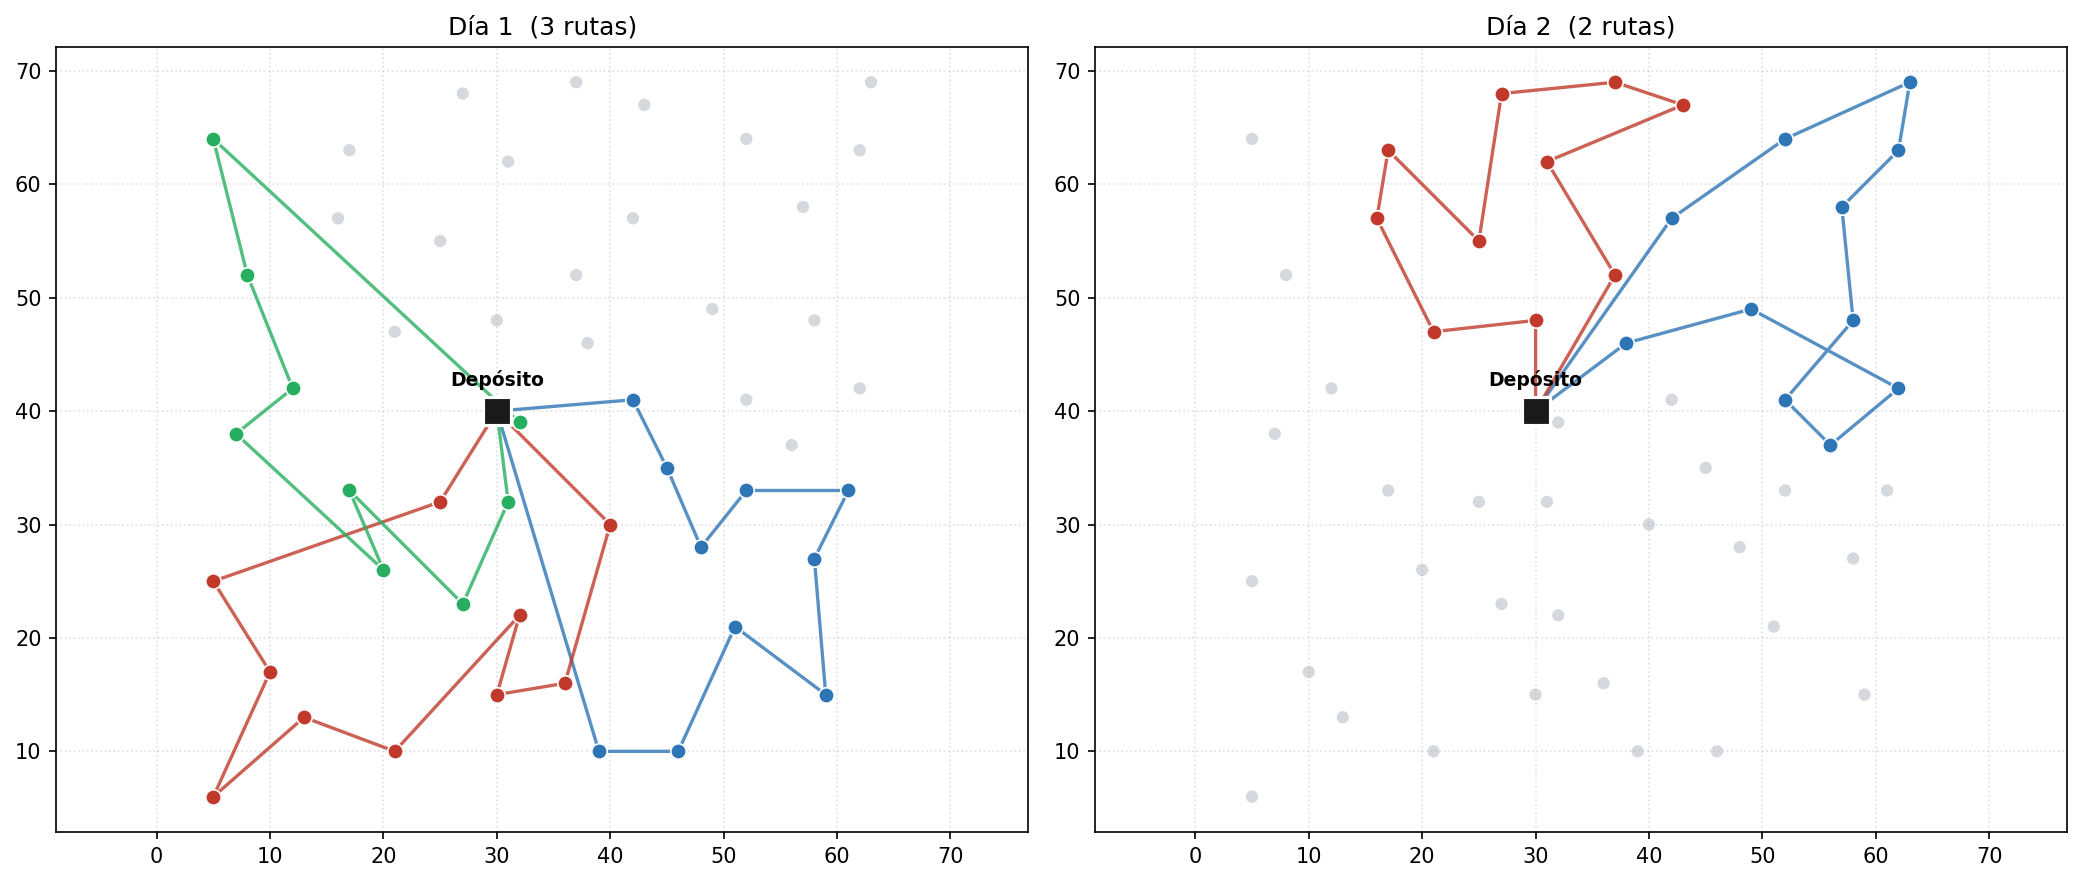
\includegraphics[width=\linewidth]{figures/rutas_p01_RL.png}
            \caption{Solución generada por el agente RL: Costo $617.4$, factible.}
        \end{subfigure}

        \begin{subfigure}{0.95\textwidth}
            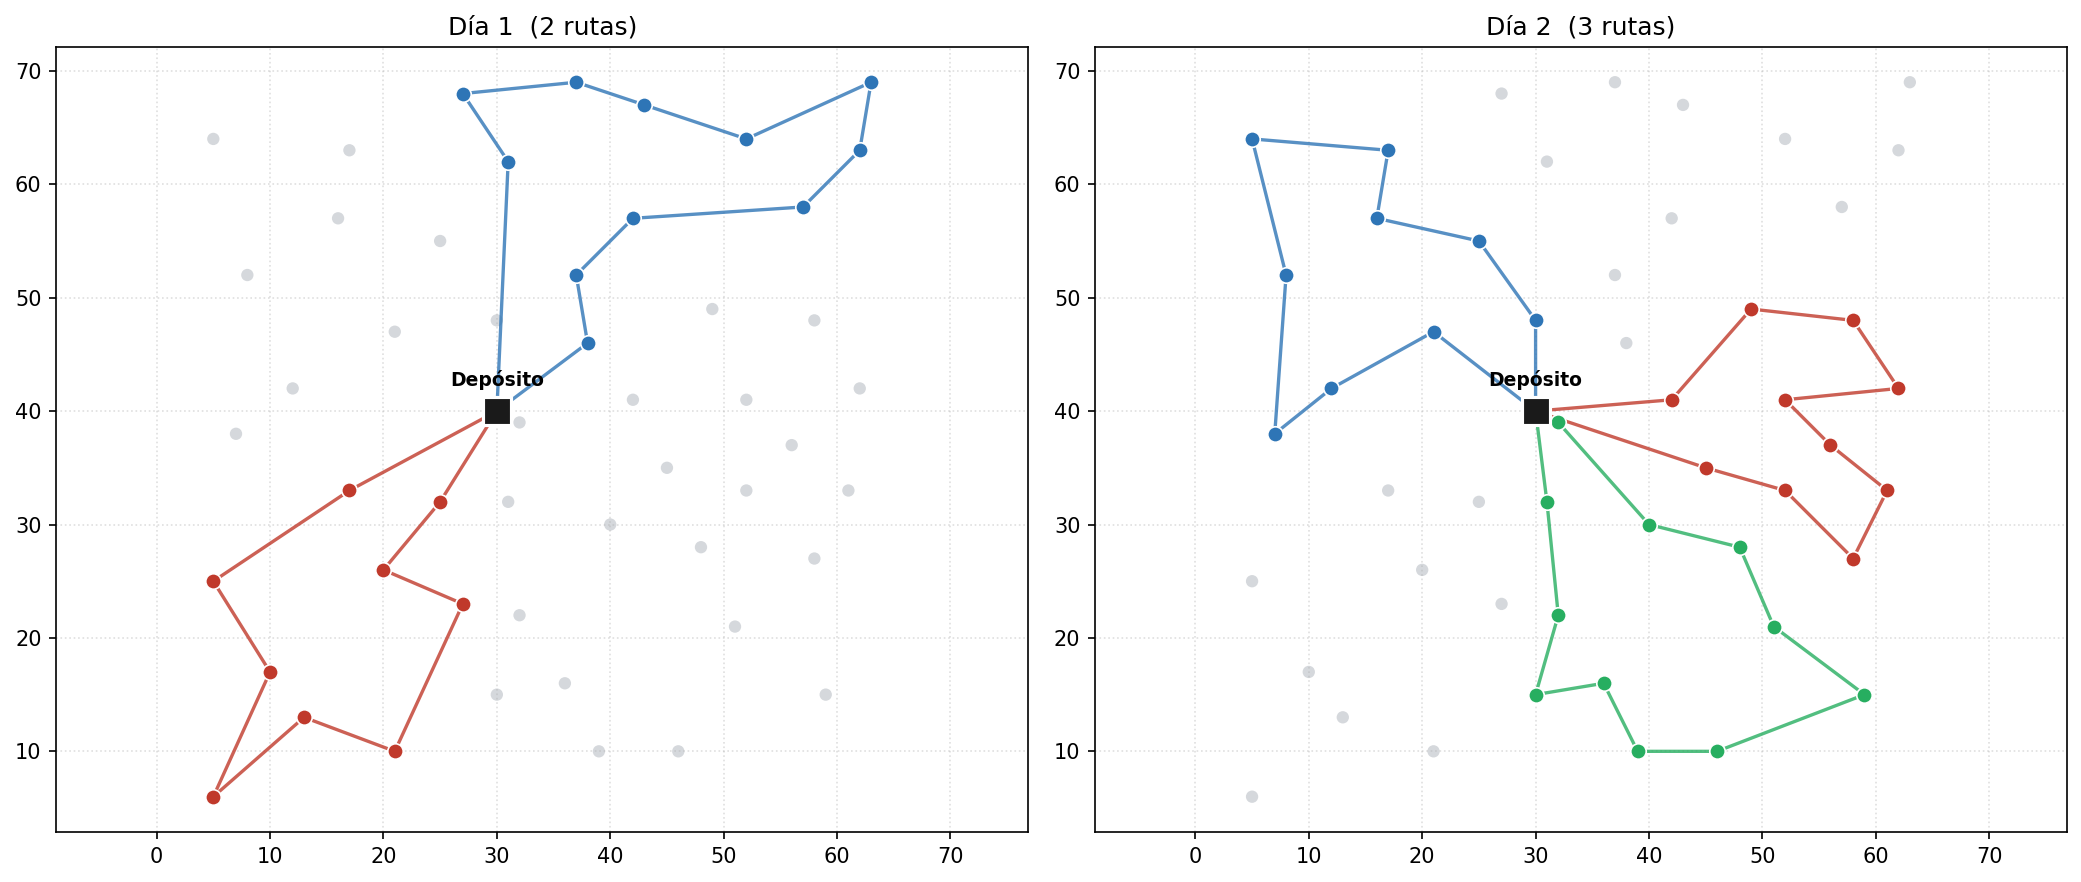
\includegraphics[width=\linewidth]{figures/rutas_p01_BKS.png}
            \caption{Mejor solución conocida BKS: Costo $524.6$.}
        \end{subfigure}
    \end{minipage}
    \caption{Rutas en la instancia $p01$.}
    \caption*{Fuente: Elaboración propia.}
    \label{fig:rutas-p01}
\end{figure}

Ambas soluciones logran agrupar a los clientes en zonas lógicas, pero la ruta del agente muestra algunos cruces de aristas que la mejor solución conocida logra evitar. Esto explica visualmente por qué existe ese gap. Tal como evidencia la figura, el agente es capaz de aprender la estructura global del problema, sabe qué clientes asignar a cada día y cómo agruparlos por vehículo, pero al construir la ruta paso a paso de forma secuencial, inevitablemente deja pequeños cruces que una heurística de mejora local sí limpiaría. Este patrón refleja una limitación inherente al enfoque constructivo puro y motiva las líneas de trabajo futuro.

\javi{Profe, respondo: (1) p01 es el caso principal porque fue la instancia sobre la que desarrollé y calibré el modelo, por su escala reducida y estructura simple. (2) El tiempo es de inferencia (agente ya entrenado construyendo la solución), no de entrenamiento. (3) La figura muestra una solución representativa del agente (costo 617,4), no la mejor; aclaré que está dentro del rango multi-semilla para que no se lea como cherry-picking. (4) Ya removí los títulos y ejes de los gráficos.}

%=============================================================%
\subsection{Resultados del escalamiento a $75$ y $100$ clientes} \label{sec:resultadosescalamiento}
%=============================================================%
Para evaluar si el método escala estructuralmente a instancias mayores, el agente se enfrentó a instancias de $75$ clientes ($p04$ de la familia A y $p06$ de la familia C) y de $100$ clientes ($p07$ de la familia A y $p09$ de la familia C), utilizando la configuración de red ampliada ($[512,512]$, $500\,000$ pasos). La Tabla~\ref{tab:escalamiento} consolida estos resultados, incluyendo también las instancias base de $50$ clientes ($p01$ y $p03$) para dimensionar el impacto del escalamiento. Esta tabla se centra deliberadamente en el contraste entre el agente RL y el VNS, su rival principal; los datos completos de la heurística Greedy, los costos absolutos, el BKS y los tiempos de ejecución para todas las instancias se reportan de forma integral en las Tablas~\ref{tab:consolidada} y~\ref{tab:tiempos} de la Sección~\ref{sec:comparacion-global}. \eli{¿no hay Greedy ni BKS ni tiempos?} \javi{Profe, esta tabla la dejé enfocada en RL vs VNS a propósito, para mostrar la degradación al escalar sin saturarla. Greedy, BKS y tiempos están completos en las tablas consolidadas de la Sección de comparación global (Tablas~\ref{tab:consolidada} y~\ref{tab:tiempos}).}

\begin{table}[H]
    \centering
    \caption{\label{tab:escalamiento} Resultados del escalamiento del agente a instancias de $75$ y $100$ clientes. Gap reportado como media $\pm$ desviación estándar sobre semillas factibles.}
    \caption*{Fuente: Elaboración propia.}
    \small
    \renewcommand{\arraystretch}{1.15}
    \setlength{\tabcolsep}{7pt}
    \begin{tabular}{@{}cccccc@{}}
        \toprule
        \textbf{Familia} & \textbf{Instancia} & \textbf{Clientes} & \textbf{Gap RL (\%)} & \textbf{Factibilidad} & \textbf{Gap VNS (\%)} \\
        \midrule
        \multirow{3}{*}{A} & $p01$ &  $50$ & $+19{,}7 \pm 6{,}5$ & $5/5$ & $+31{,}7$ \\
                           & $p04$ &  $75$ & $+53{,}9 \pm 5{,}4$ & $5/5$ & $+23{,}1$ \\
                           & $p07$ & $100$ & $+57{,}4 \pm 6{,}5$ & $5/5$ & $+27{,}3$ \\
        \midrule
        \multirow{3}{*}{C} & $p03$ &  $50$ & $+28{,}0 \pm 5{,}3$ & $5/5$ & $+83{,}8$ \\
                           & $p06$ &  $75$ & $+55{,}7 \pm 2{,}4$ & $4/5$ & $+104{,}7$ \\
                           & $p09$ & $100$ & $+66{,}7 \pm 5{,}7$ & $5/5$ & $+128{,}5$ \\
        \bottomrule
    \end{tabular}
\end{table}

El análisis de estos datos arroja tres observaciones clave. Primero, la factibilidad se mantiene en niveles sumamente altos en todas las escalas ($29$ de $30$ corridas factibles, logrando una tasa global del $97\%$), incluso al duplicar el número de clientes y aumentar el horizonte de planificación. Segundo, aunque la calidad respecto al BKS disminuye al crecer la instancia, esta degradación resulta suave y predecible: el mayor salto ocurre al pasar de $50$ a $75$ clientes, mientras que entre $75$ y $100$ el gap tiende a estabilizarse. Tercero, la pérdida de calidad es muy similar entre las familias A y C a igual escala, lo que demuestra que el rendimiento del modelo depende mucho más del tamaño del estado que de las restricciones temporales específicas de cada familia.

La Figura~\ref{fig:evolucion-gap} ilustra este patrón. El gráfico muestra la evolución del gap medio respecto al BKS en función del número de clientes, tanto para el agente RL (familias A y C) como para VNS (familia A). Aquí queda en evidencia que el agente RL experimenta un salto pronunciado en el gap entre $50$ y $75$ clientes, seguido de una estabilización hacia los $100$. En contraste, la heurística VNS logra mantener gaps casi constantes en la familia A a lo largo de las tres escalas.

\begin{figure}[H]
    \centering
    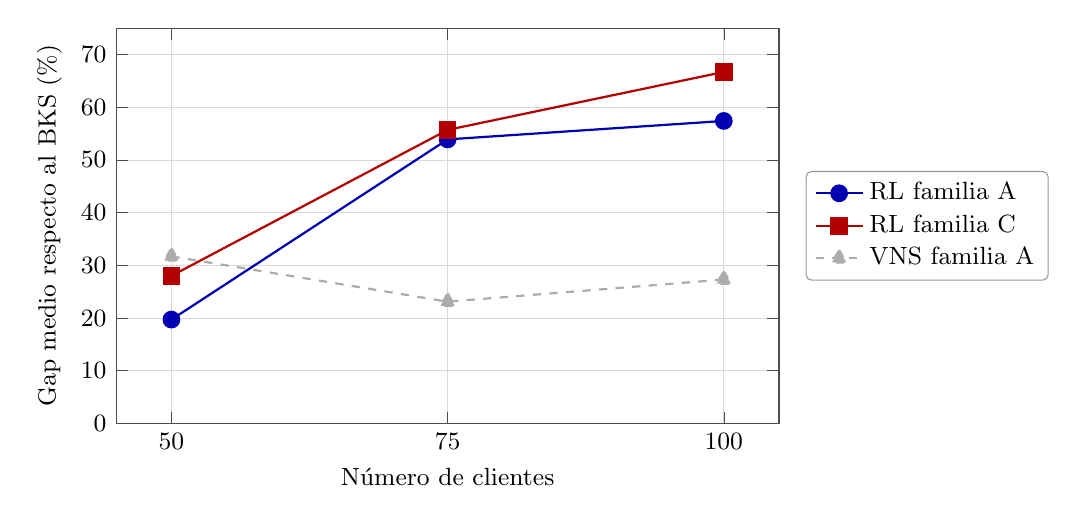
\begin{tikzpicture}
        \begin{axis}[
            width=10cm,
            height=6.6cm,
            xlabel={Número de clientes},
            ylabel={Gap medio respecto al BKS (\%)},
            xmin=45, xmax=105,
            ymin=0, ymax=75,
            xtick={50,75,100},
            ytick={0,10,20,30,40,50,60,70},
            grid=major,
            xmajorgrids=true,
            ymajorgrids=true,
            grid style={line width=0.3pt, draw=gray!30},
            axis line style={black!70},
            tick style={black!70},
            tick label style={font=\small},
            label style={font=\small},
            legend style={
                font=\small,
                draw=black!40,
                fill=white,
                rounded corners=2pt,
                at={(1.04,0.5)},
                anchor=west
            },
            legend cell align=left,
            clip=false
        ]
            \addplot[color=blue!70!black, thick, mark=*, mark size=2.8pt]
            coordinates {(50,19.7) (75,53.9) (100,57.4)};
            \addlegendentry{RL familia A}

            \addplot[color=red!70!black, thick, mark=square*, mark size=2.8pt]
            coordinates {(50,28.0) (75,55.7) (100,66.7)};
            \addlegendentry{RL familia C}

            \addplot[color=gray!65, thick, dashed, mark=triangle*, mark size=3pt]
            coordinates {(50,31.7) (75,23.1) (100,27.3)};
            \addlegendentry{VNS familia A}
        \end{axis}
    \end{tikzpicture}
    \caption{Evolución del gap medio respecto al BKS según el número de clientes.}
    \caption*{Fuente: Elaboración propia.}
    \label{fig:evolucion-gap}
\end{figure}

Para complementar los números con evidencia visual, las Figuras~\ref{fig:rutas-p03} a~\ref{fig:rutas-p09-bks} contrastan soluciones representativas construidas por el agente con las mejores soluciones conocidas, organizadas según el tamaño de la instancia ($50$, $75$ y $100$ clientes) para observar directamente el efecto del escalamiento.

Comenzando con la escala base de $50$ clientes, la Figura~\ref{fig:rutas-p03} expone la instancia $p03$ (familia C, horizonte de 5 días, un vehículo). En este escenario, el agente logra un gap de $+28{,}0\%$, superando por un amplio margen el $+83{,}8\%$ de VNS. Visualmente, se aprecia que el modelo RL genera agrupaciones sumamente limpias, con muy pocos cruces locales.

\begin{figure}[H]
    \centering
    \begin{minipage}{0.95\textwidth}
        \centering
        \begin{subfigure}{0.95\textwidth}
            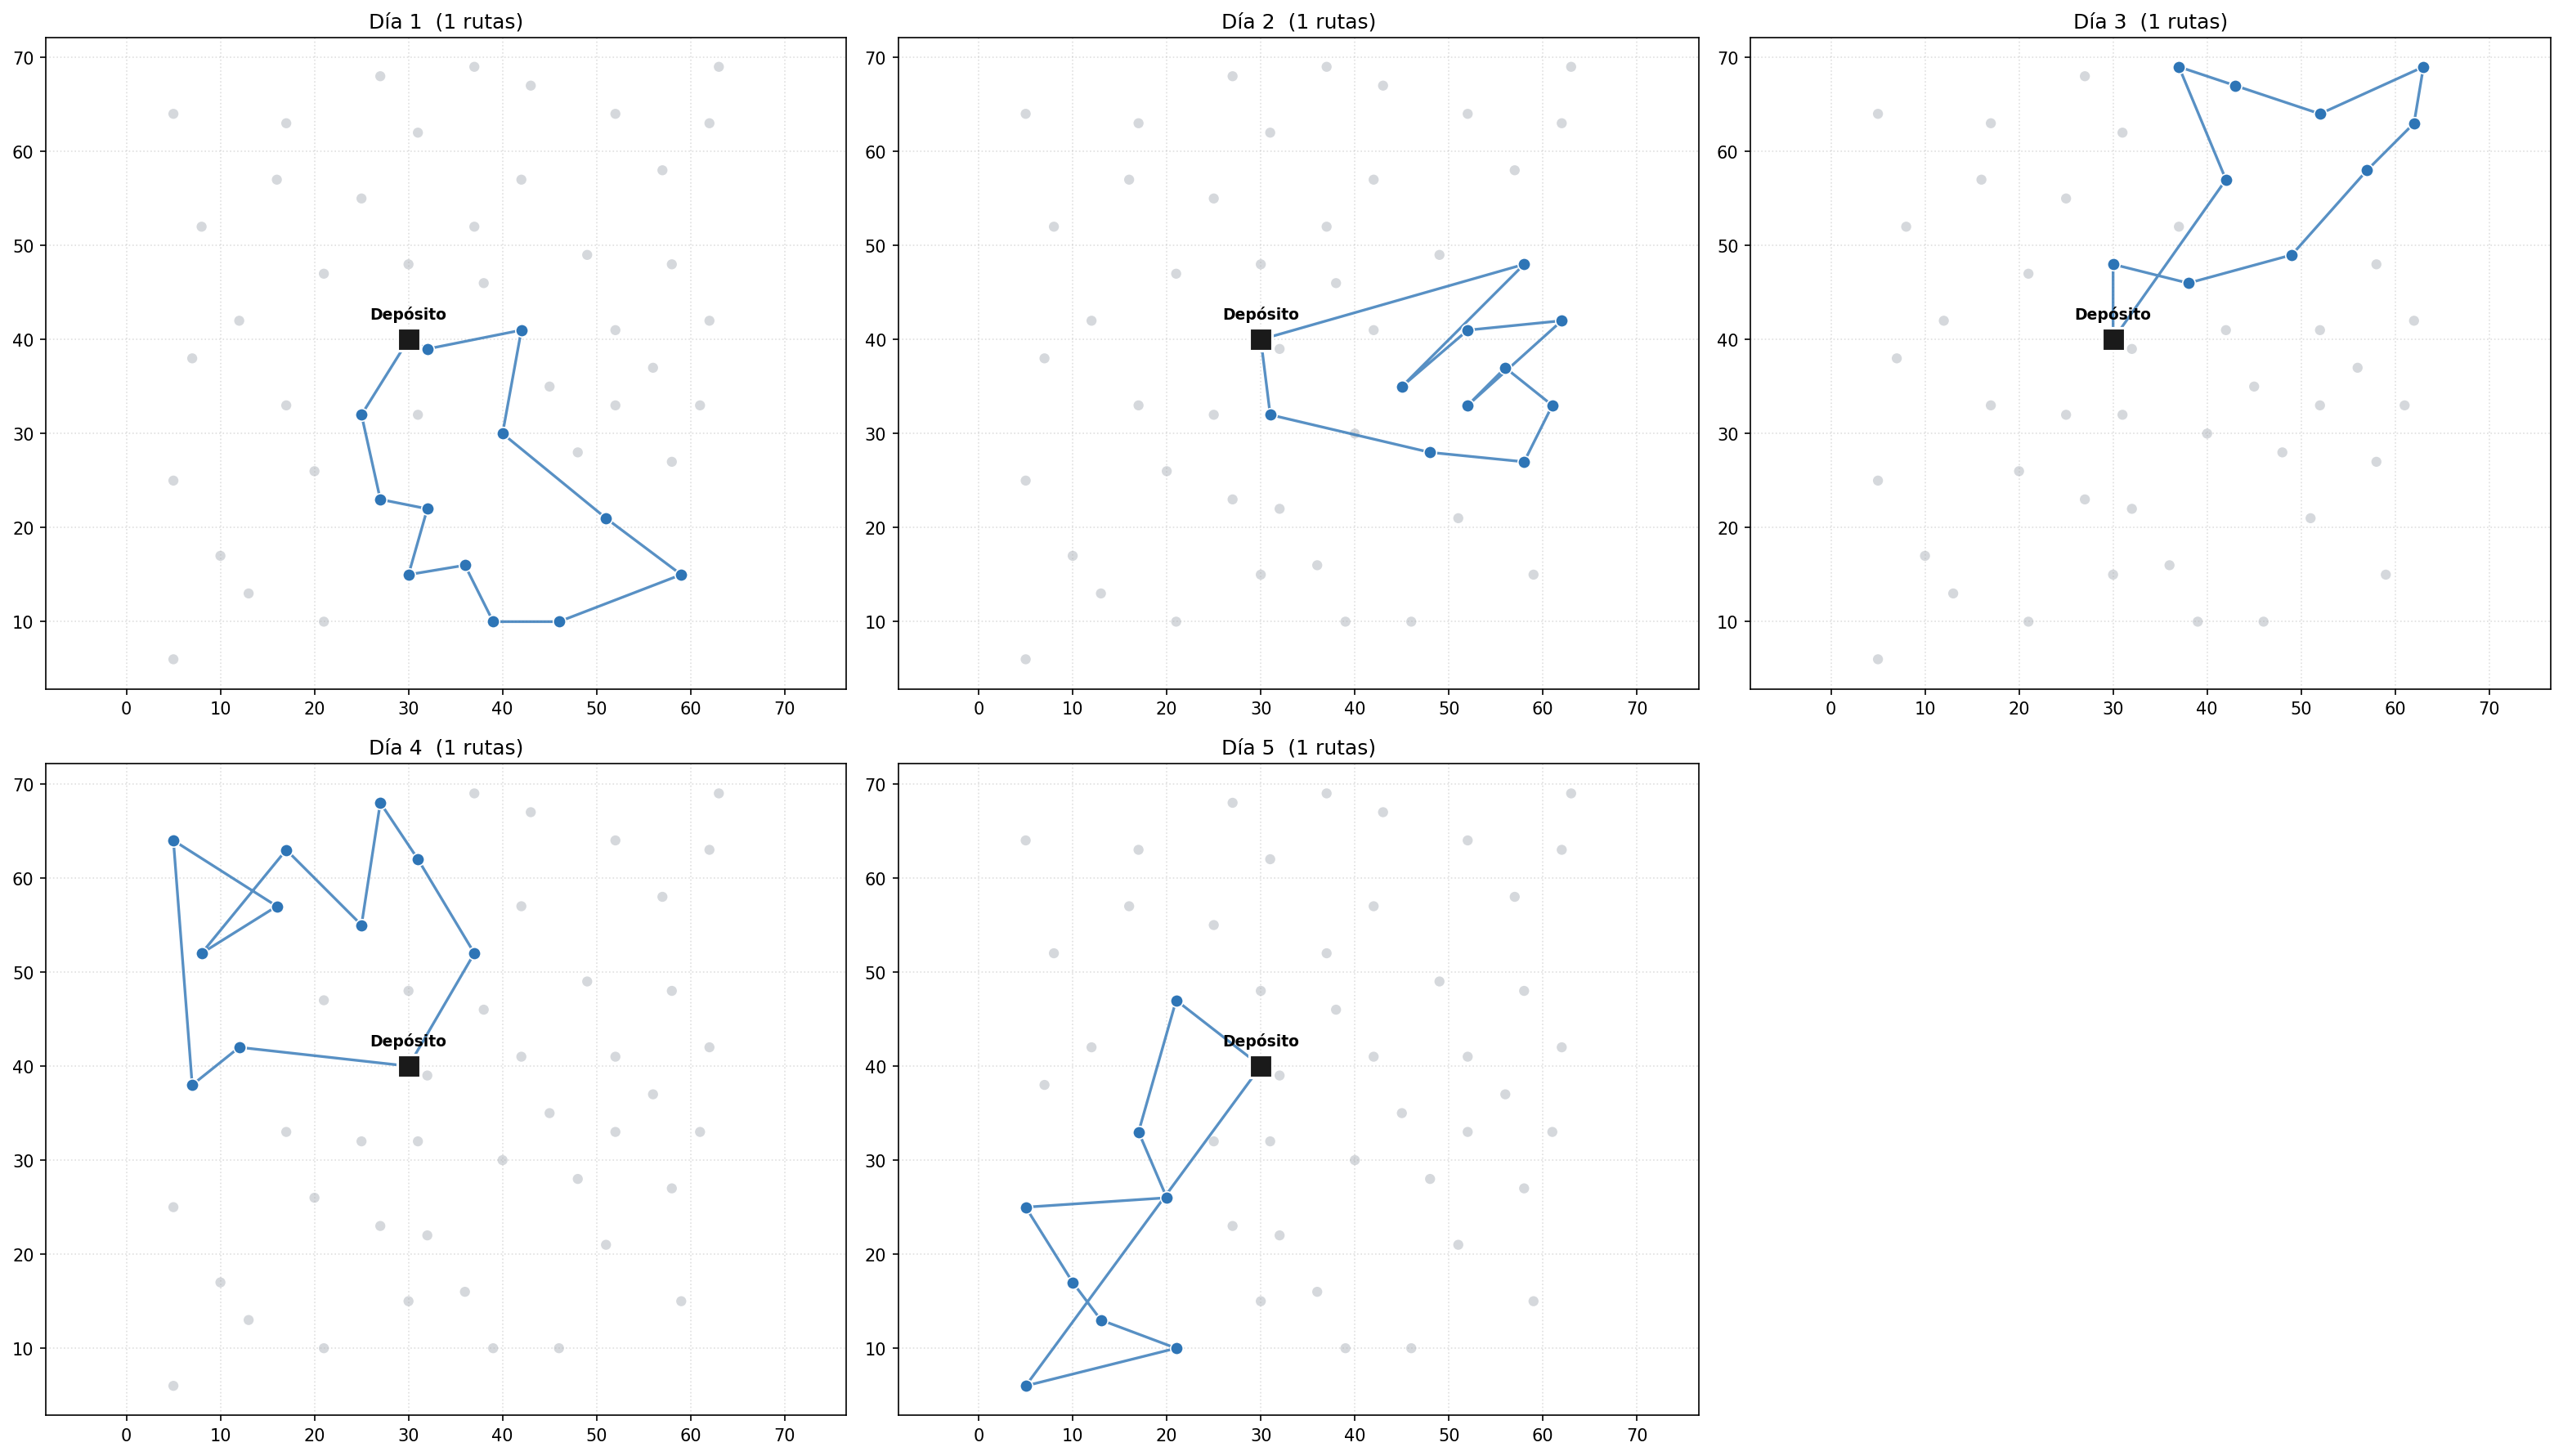
\includegraphics[width=\linewidth]{figures/rutas_p03_RL.png}
            \caption{Solución generada por el agente RL: Costo $636.5$, factible.}
        \end{subfigure}

        \begin{subfigure}{0.95\textwidth}
            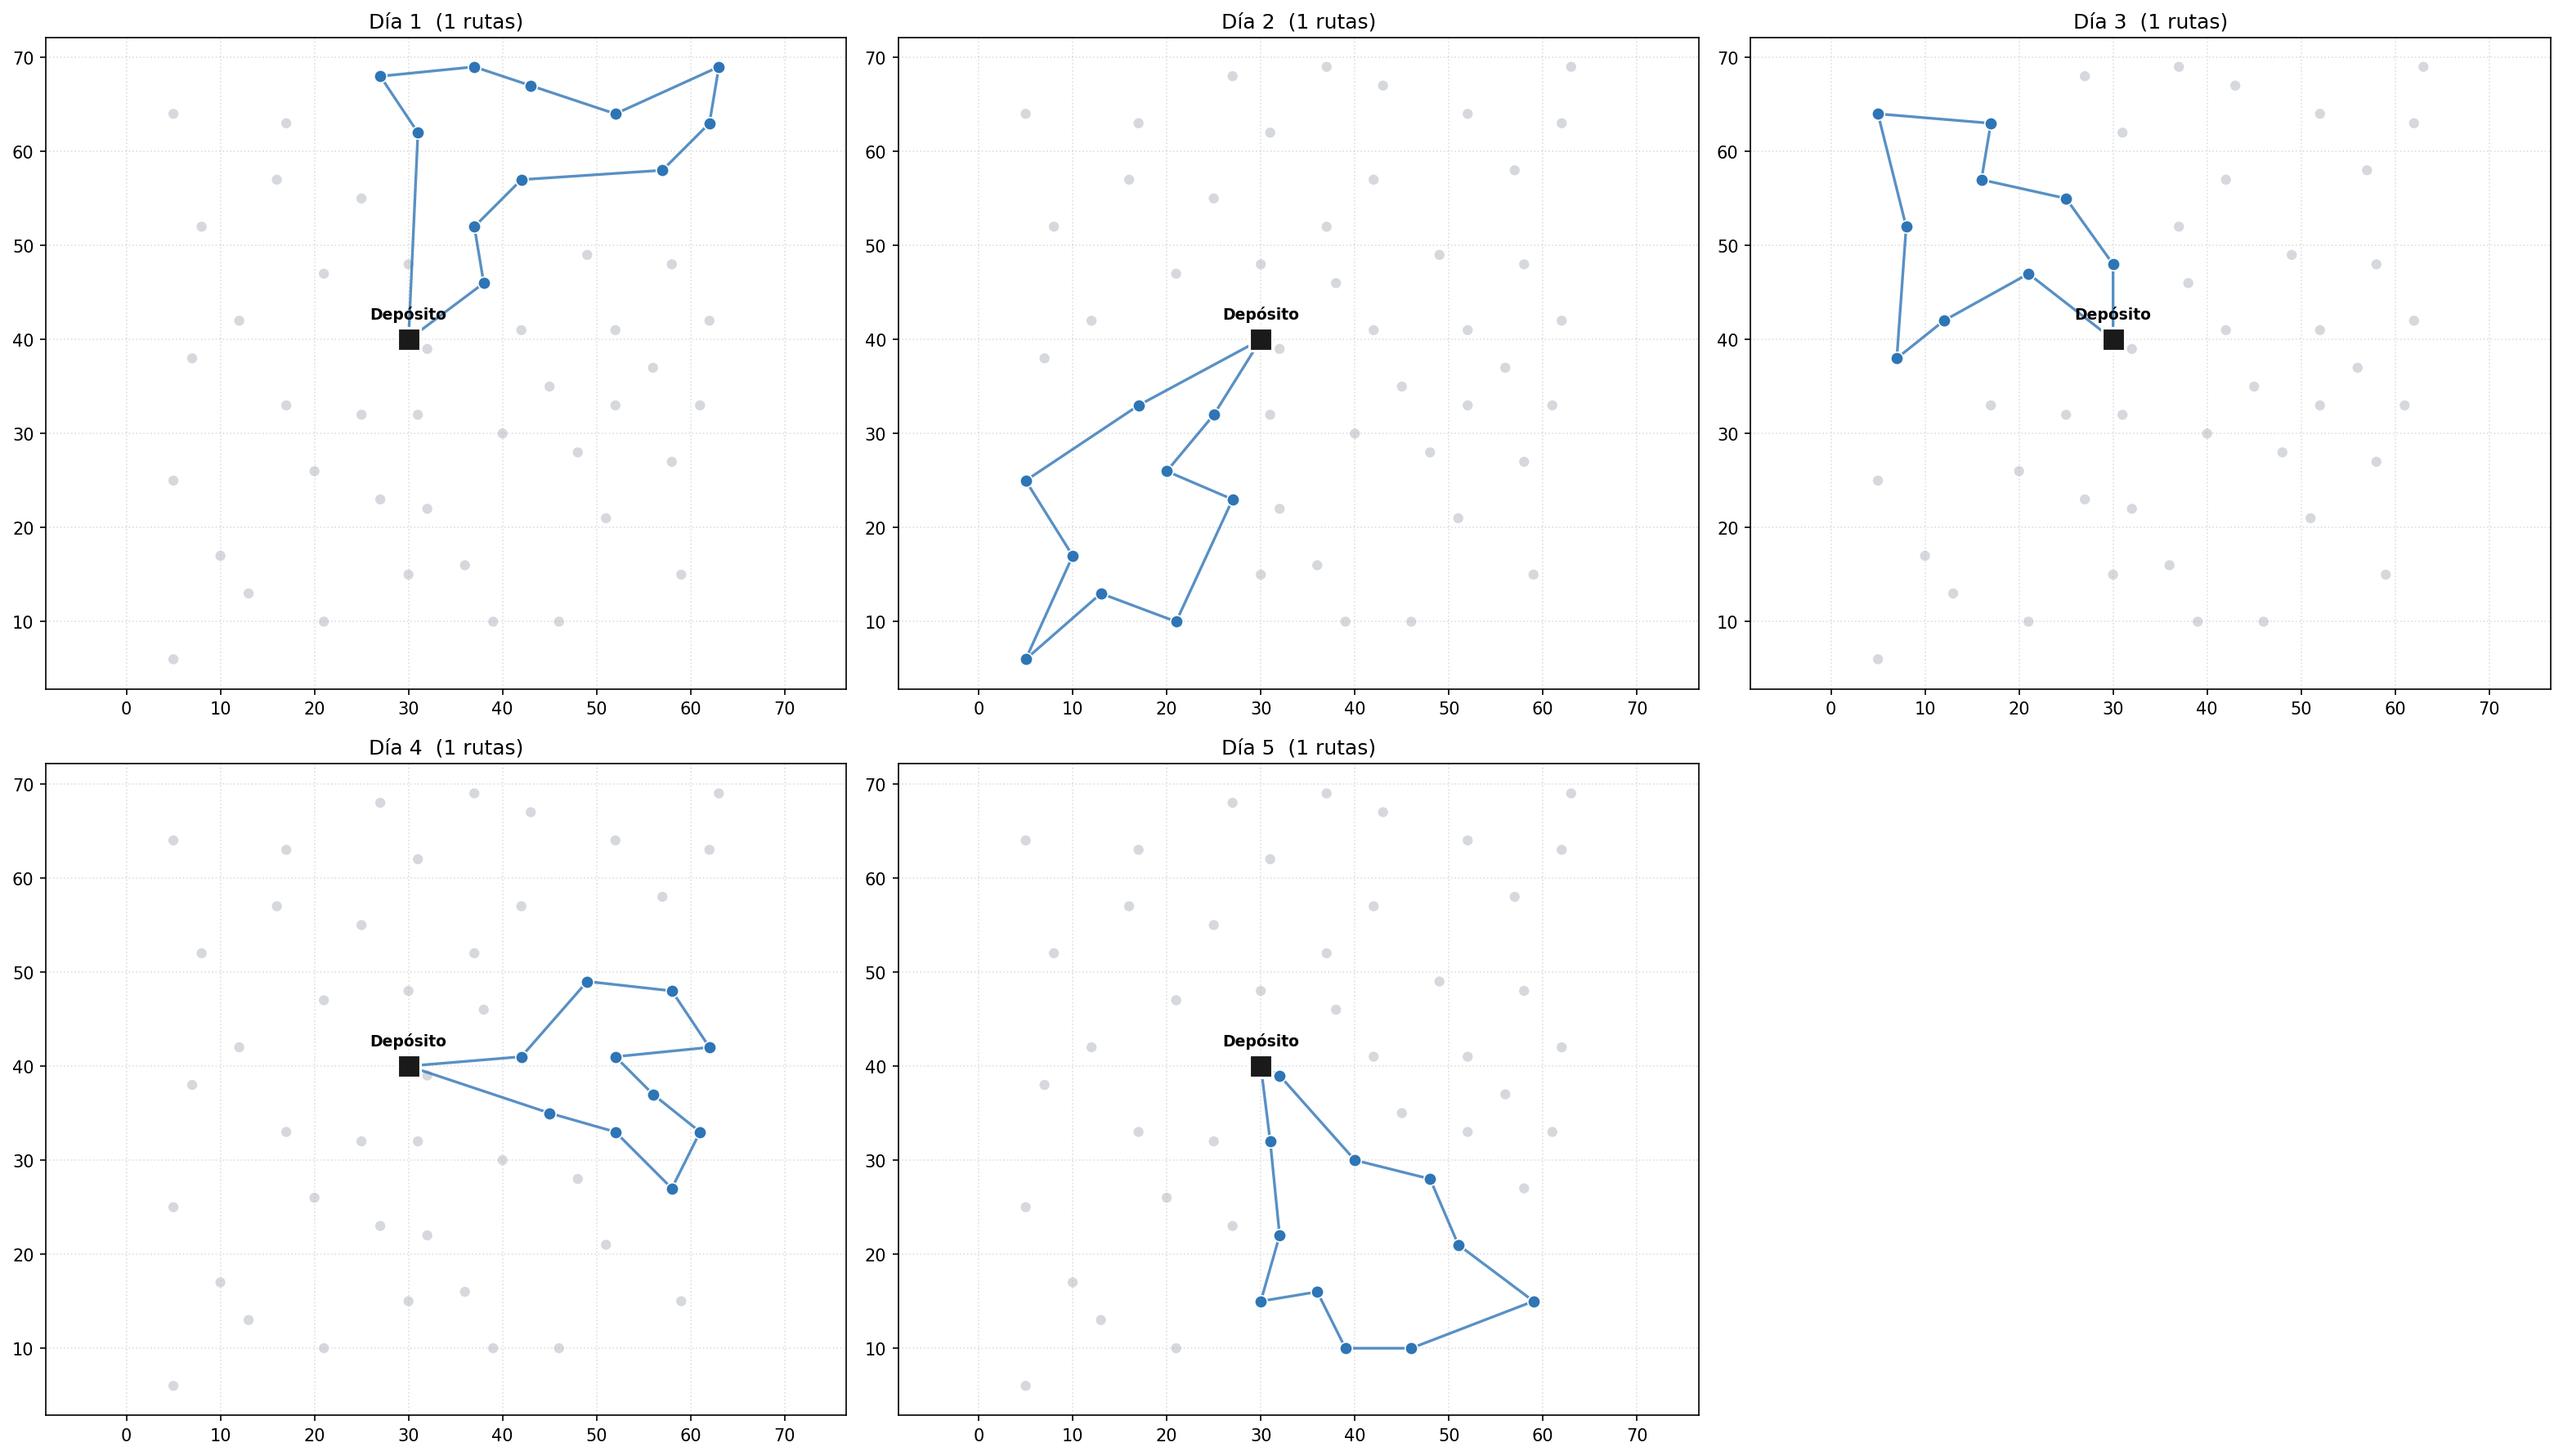
\includegraphics[width=\linewidth]{figures/rutas_p03_BKS.png}
            \caption{Mejor solución conocida BKS: Costo $524.6$.}
        \end{subfigure}
    \end{minipage}
    \caption{Rutas en la instancia $p03$.}
    \caption*{Fuente: Elaboración propia.}
    \label{fig:rutas-p03}
\end{figure}

Al subir a la escala de $75$ clientes, las Figuras~\ref{fig:rutas-p04} y~\ref{fig:rutas-p06-rl} muestran el comportamiento en las familias A y C, respectivamente. La Figura~\ref{fig:rutas-p04} presenta los resultados de la instancia $p04$ (familia A, horizonte de 2 días, cinco vehículos), donde la mayor densidad de puntos y la cantidad de vehículos por día introducen una complejidad combinatoria superior. Por su parte, las Figuras~\ref{fig:rutas-p06-rl} y~\ref{fig:rutas-p06-bks} ilustran los resultados de la instancia $p06$ (familia C, horizonte de 10 días, un vehículo), exigiendo al agente construir una secuencia temporal muy extensa. En ambos casos, el agente mantiene una zonificación global correcta, pero el aumento de puntos provoca que los cruces de aristas locales comiencen a acumularse.

\begin{figure}[H]
    \centering
    \begin{minipage}{0.95\textwidth}
        \centering
        \begin{subfigure}{0.95\textwidth}
            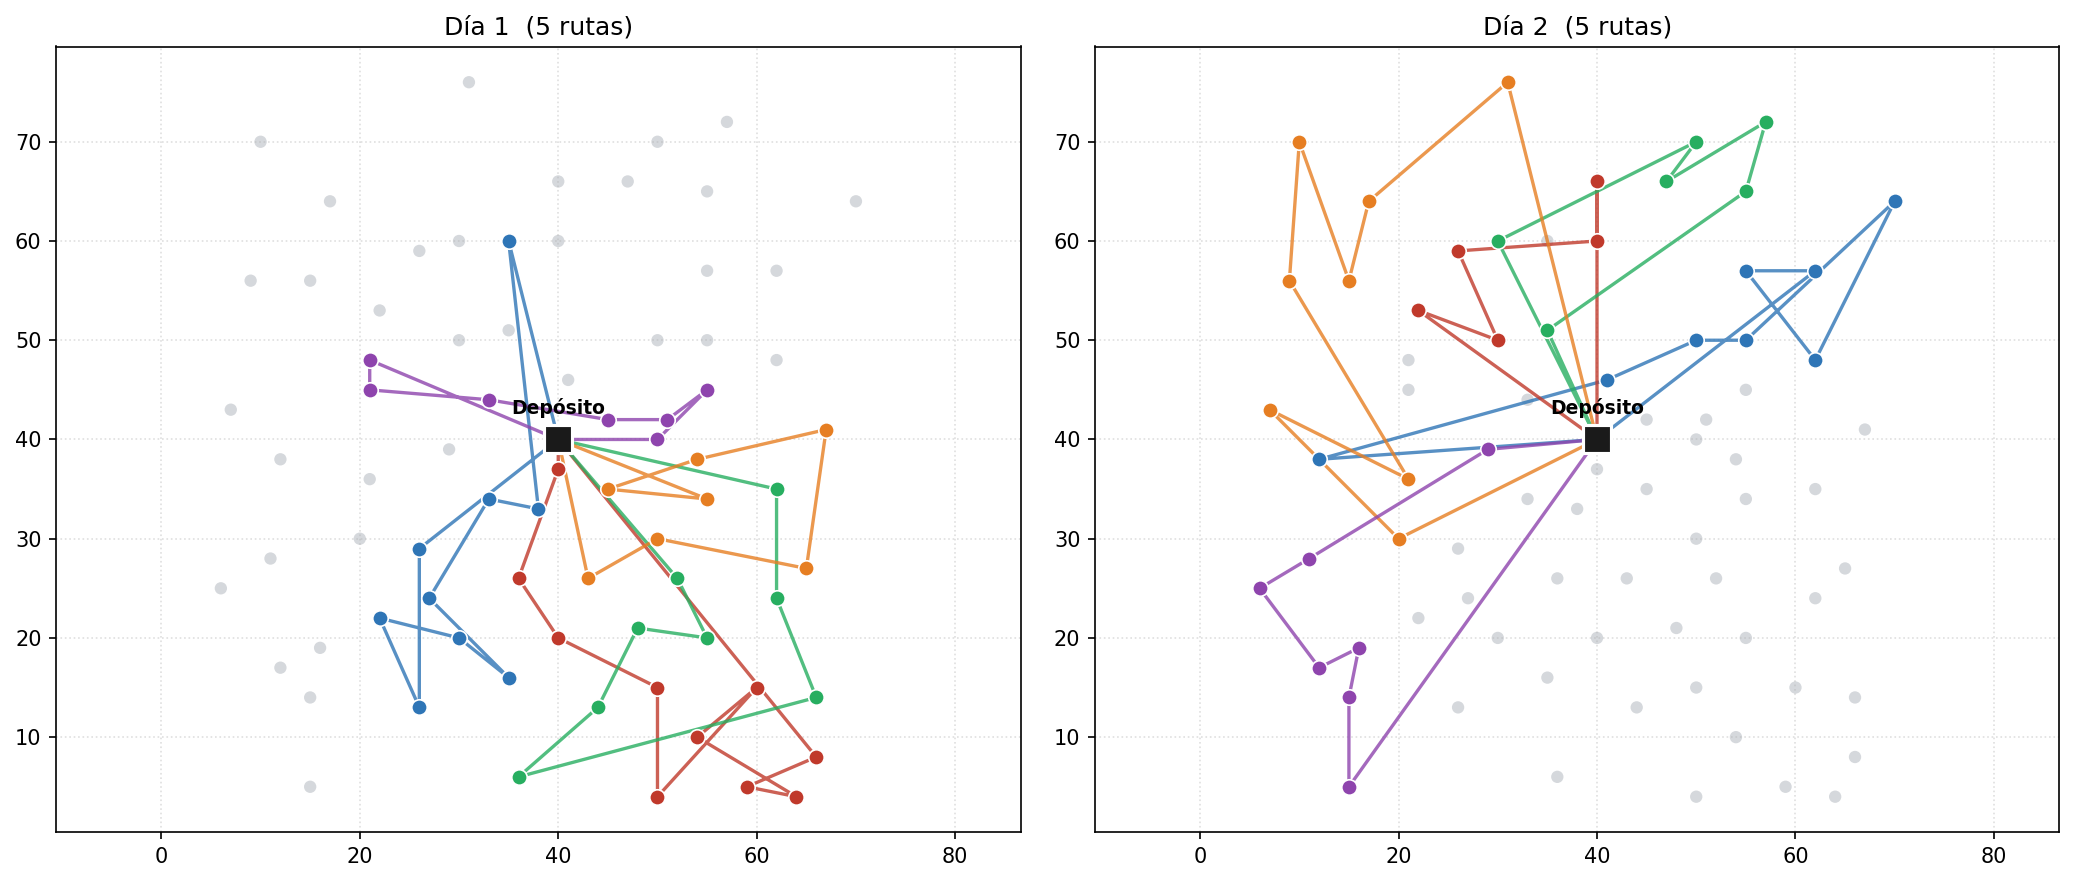
\includegraphics[width=\linewidth]{figures/rutas_p04_RL.png}
            \caption{Solución generada por el agente RL: Costo $1201.8$, factible.}
        \end{subfigure}

        \begin{subfigure}{0.95\textwidth}
            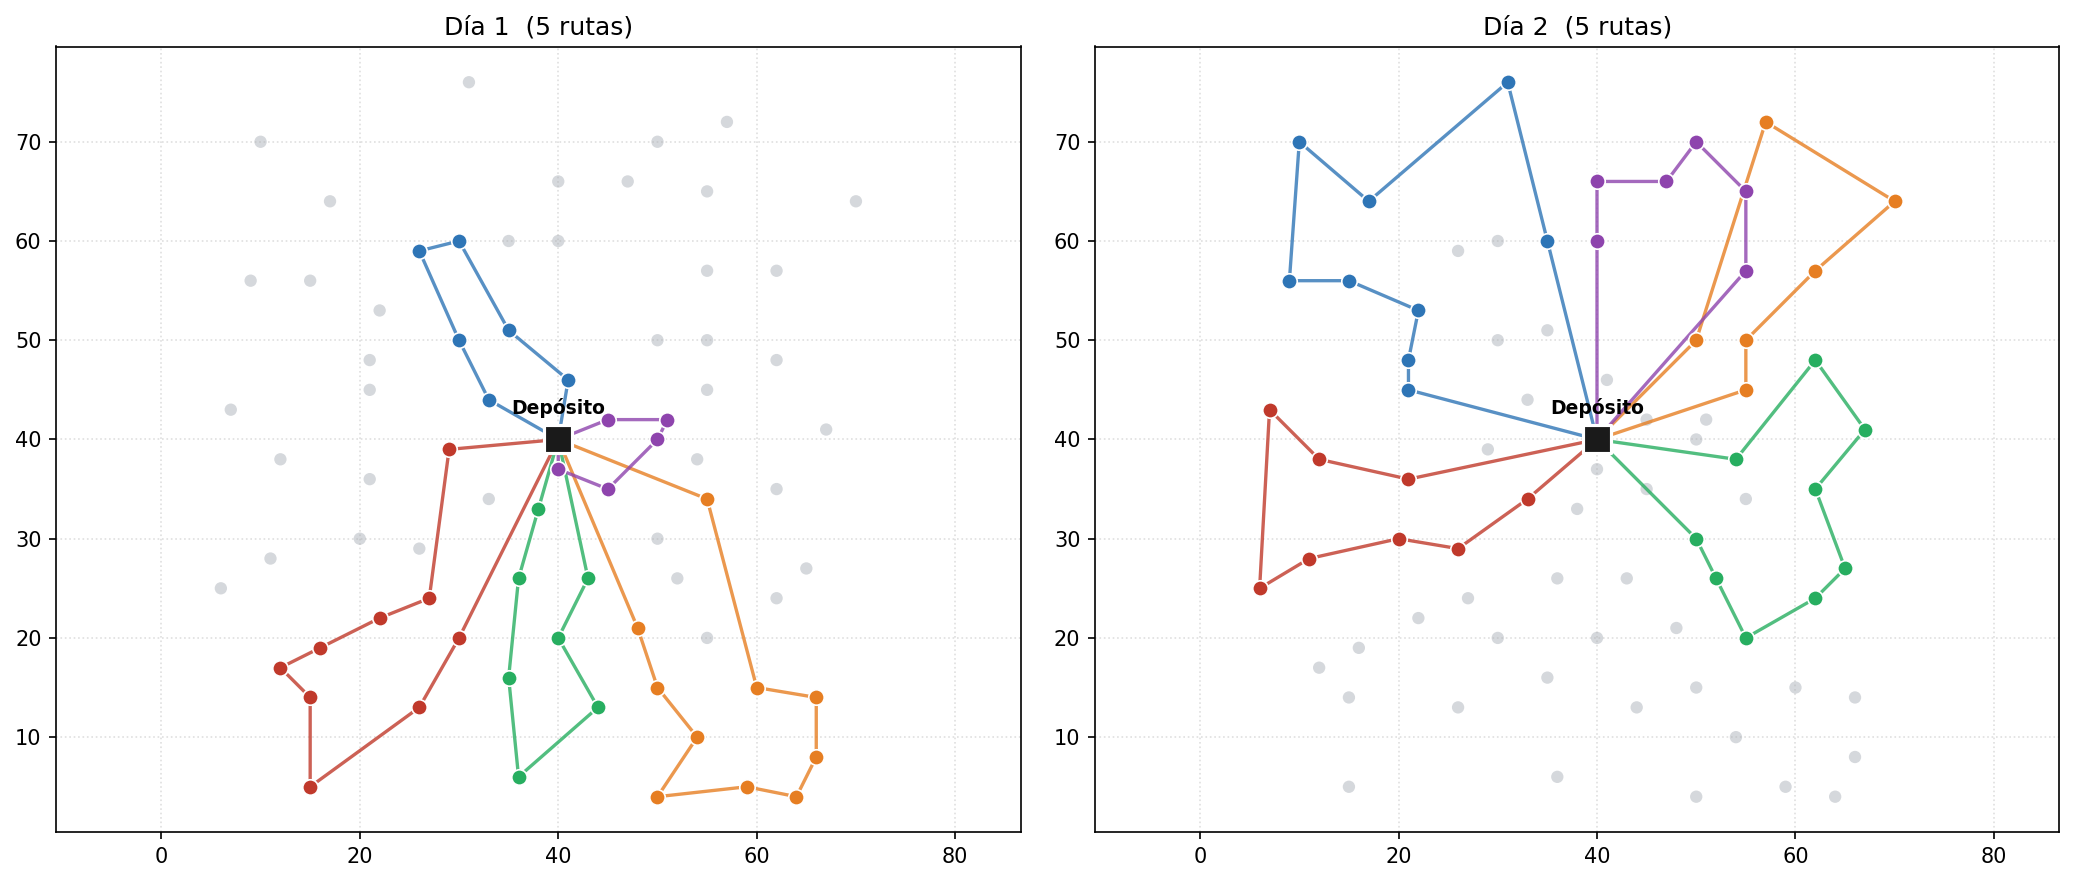
\includegraphics[width=\linewidth]{figures/rutas_p04_BKS.png}
            \caption{Mejor solución conocida BKS: Costo $835.4$.}
        \end{subfigure}
    \end{minipage}
    \caption{Rutas en la instancia $p04$.}
    \caption*{Fuente: Elaboración propia.}
    \label{fig:rutas-p04}
\end{figure}

\clearpage
\begin{figure}[H]
    \centering
    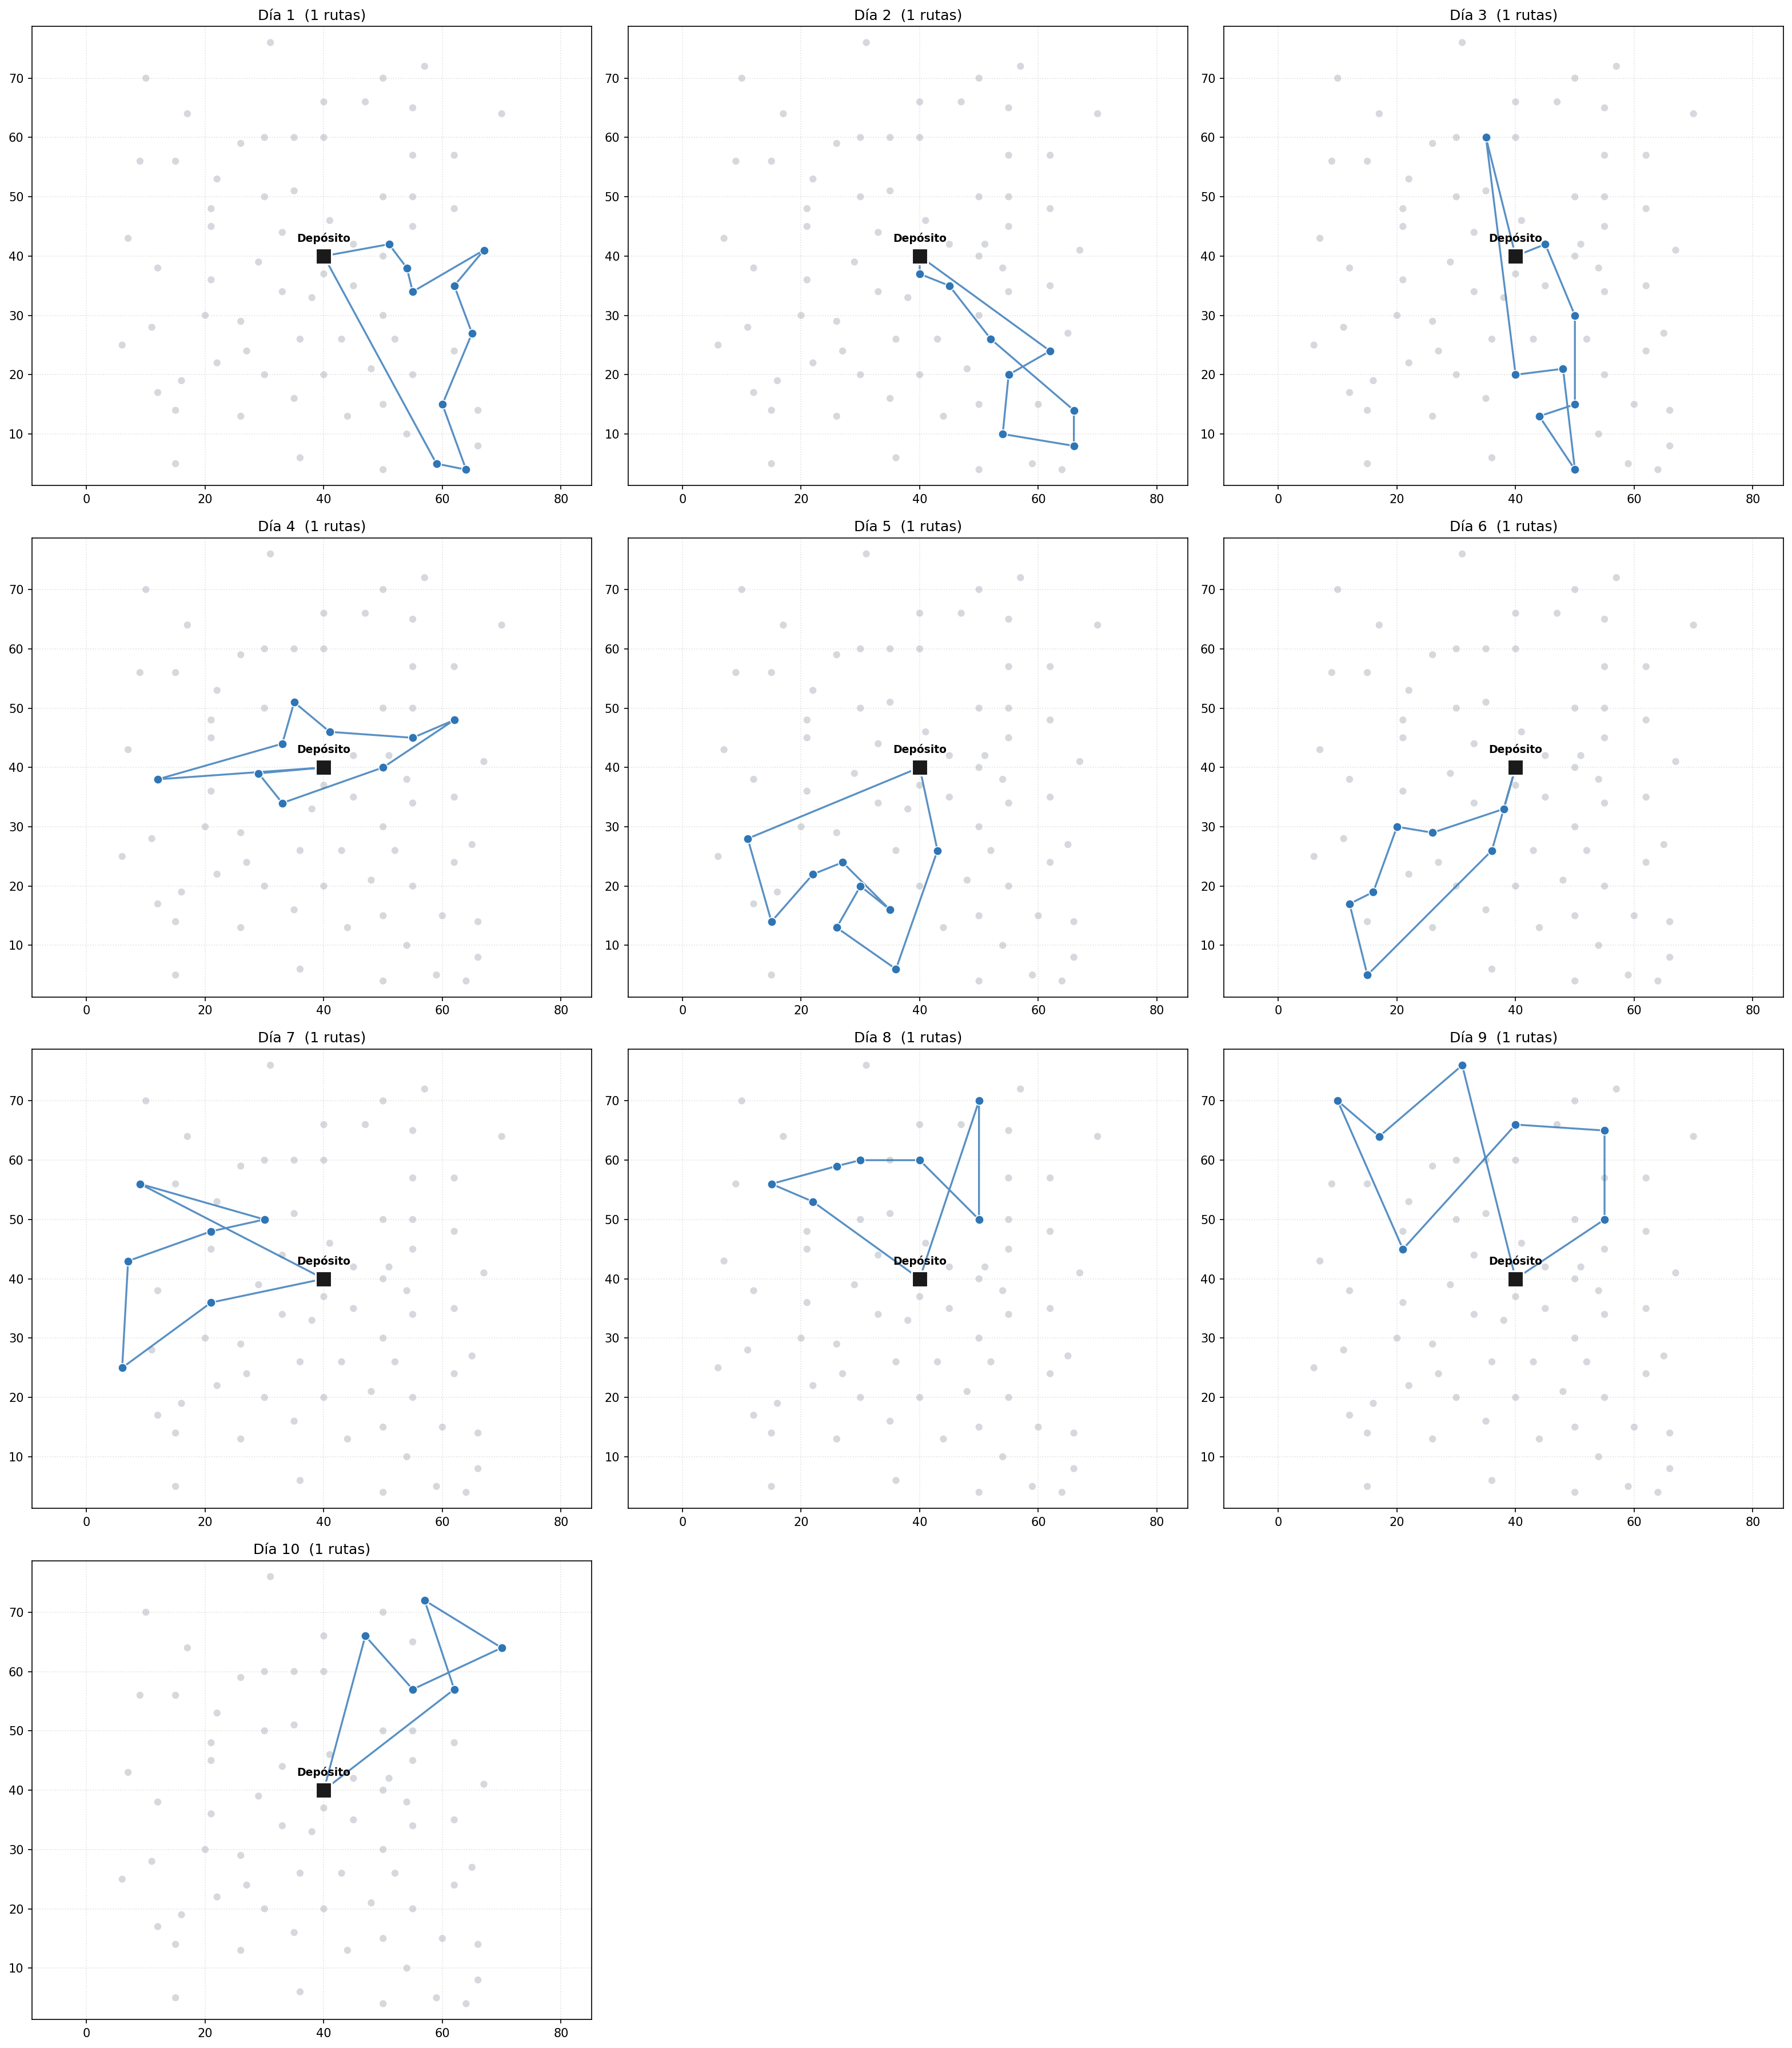
\includegraphics[
        width=\linewidth,
        height=0.80\textheight,
        keepaspectratio
    ]{figures/rutas_p06_RL.png}
    \caption{Rutas en la instancia $p06$ generadas por el agente RL: costo $1270{,}2$, factible.}
    \caption*{Fuente: Elaboración propia.}
    \label{fig:rutas-p06-rl}
\end{figure}

\clearpage
\begin{figure}[H]
    \centering
    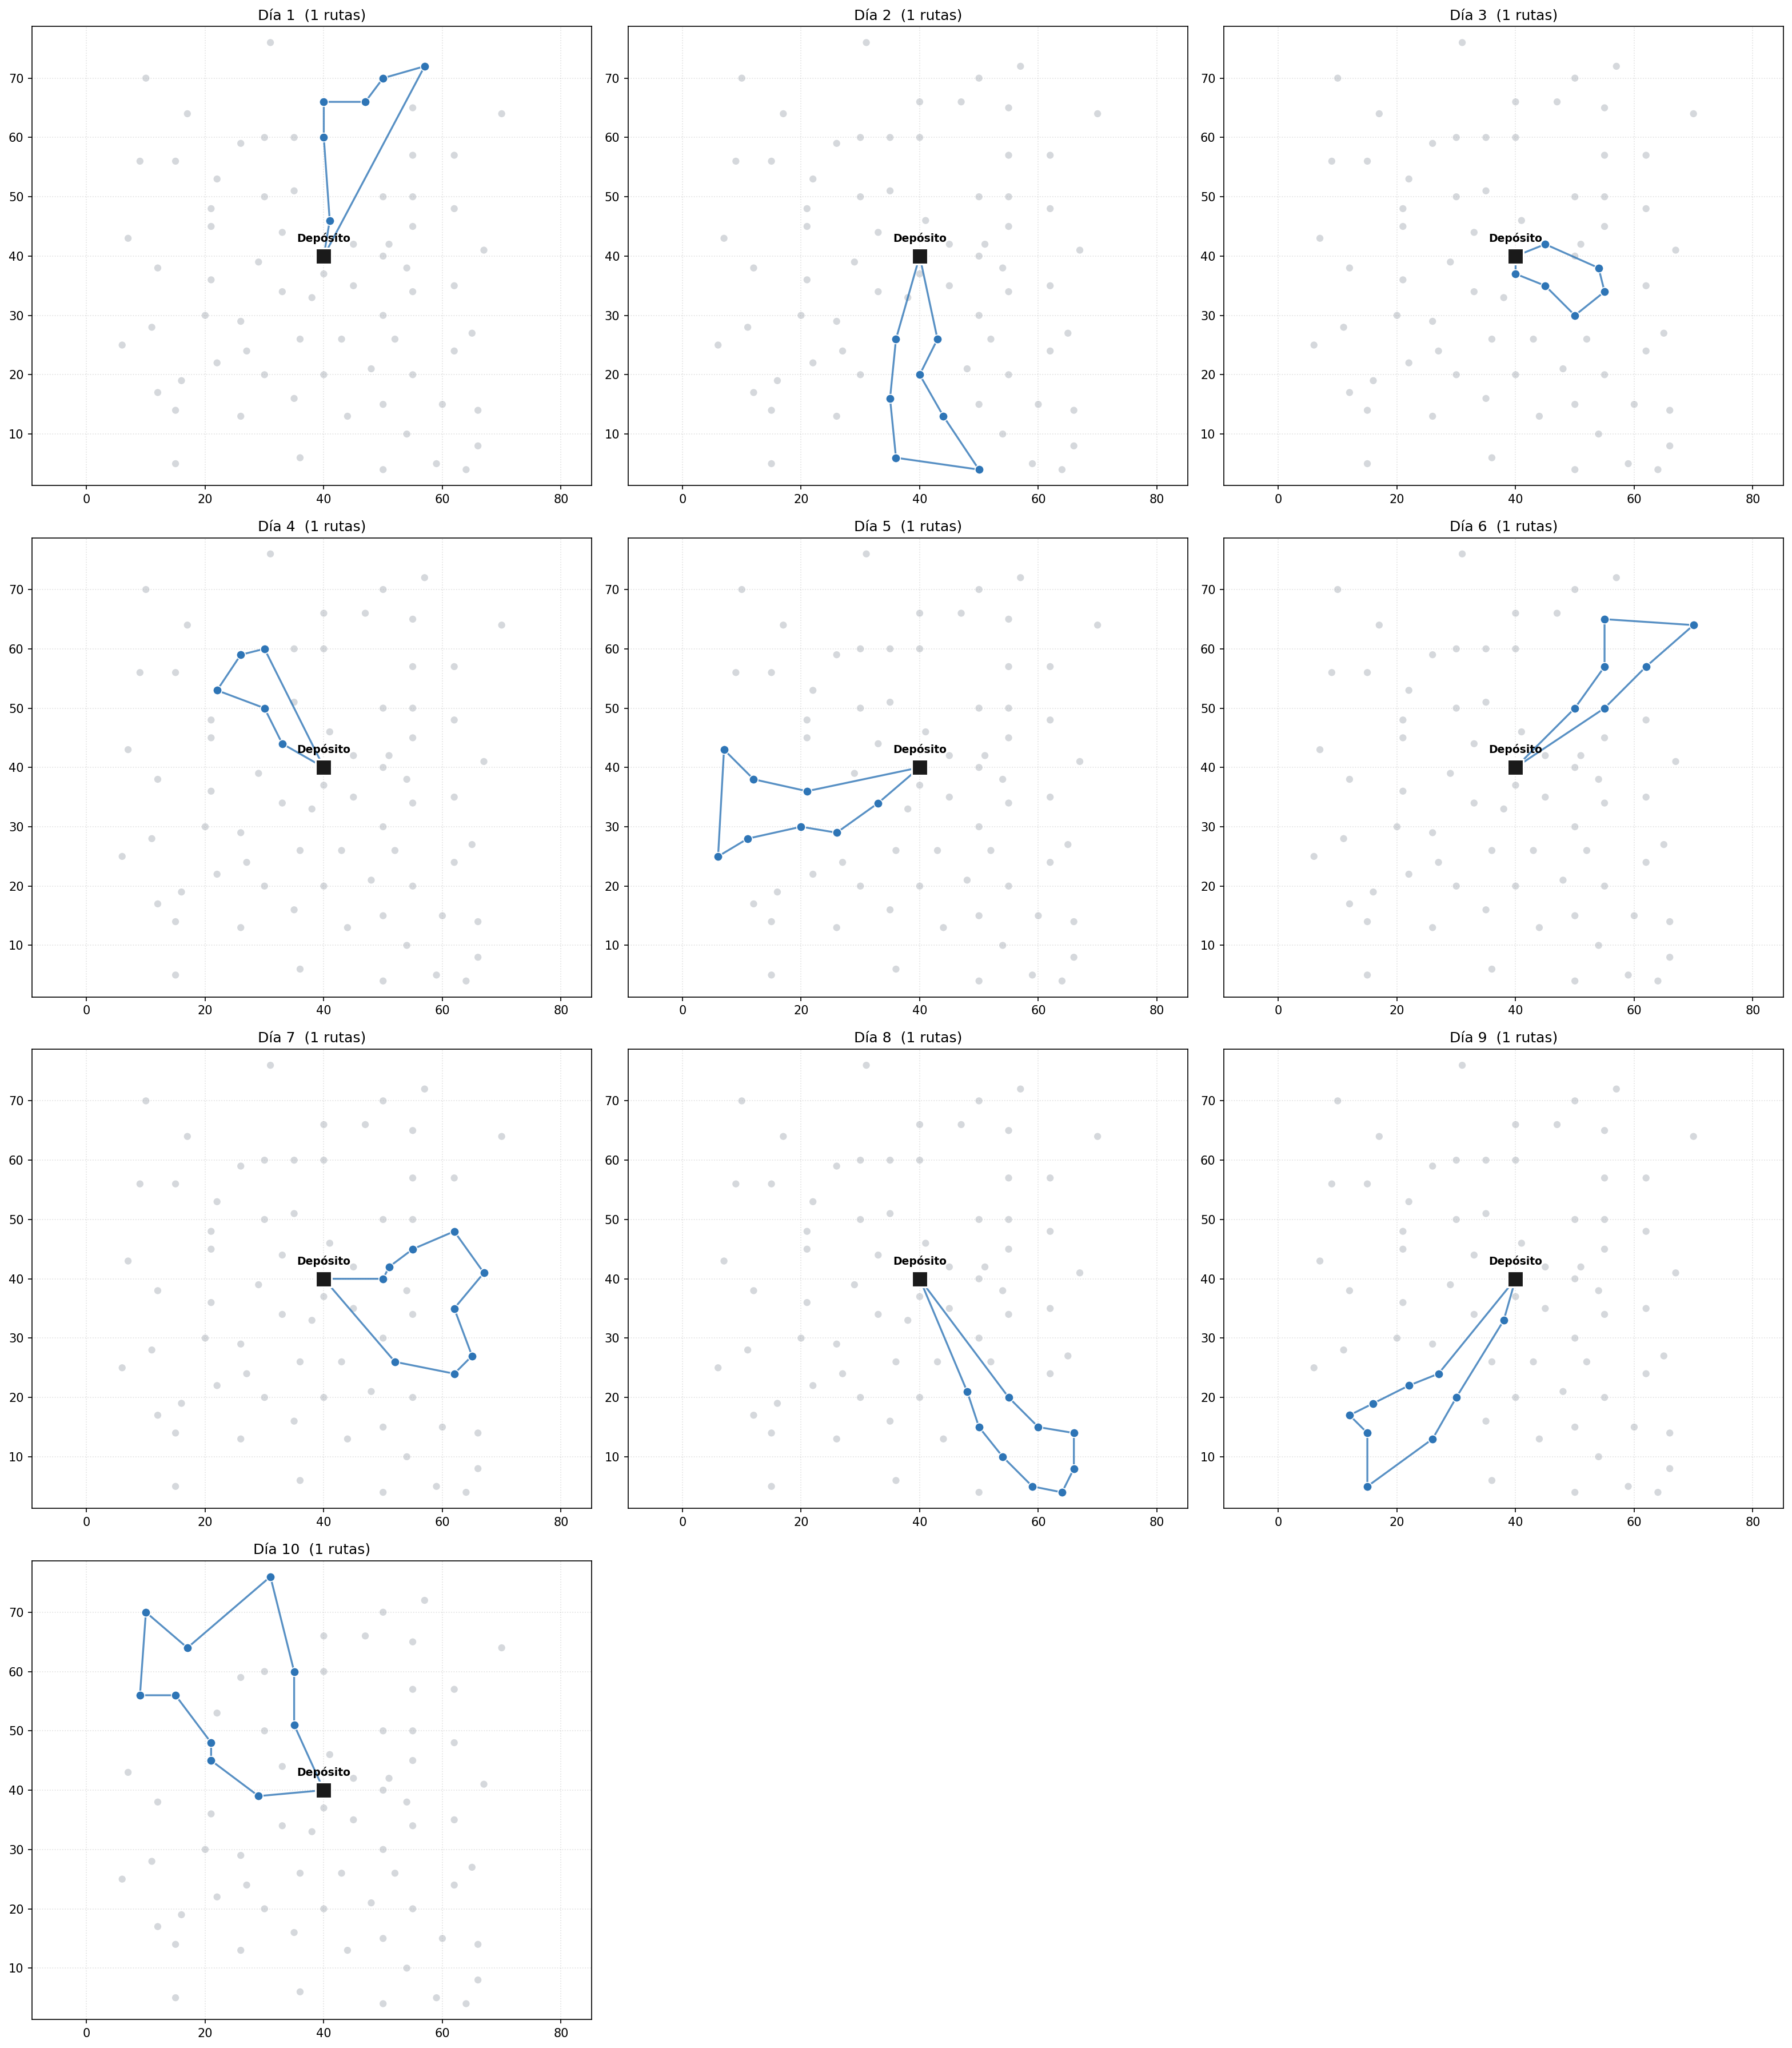
\includegraphics[
        width=\linewidth,
        height=0.80\textheight,
        keepaspectratio
    ]{figures/rutas_p06_BKS.png}
    \caption{Mejor solución conocida (BKS) para la instancia $p06$: costo $836{,}4$.}
    \caption*{Fuente: Elaboración propia.}
    \label{fig:rutas-p06-bks}
\end{figure}

Finalmente, al llegar a la escala máxima de $100$ clientes, las Figuras~\ref{fig:rutas-p07} y~\ref{fig:rutas-p09-rl} evidencian cómo el modelo maneja la mayor densidad geométrica posible del estudio. La Figura~\ref{fig:rutas-p07} presenta los resultados de la instancia $p07$ (familia A, horizonte de 2 días, cuatro vehículos), y las Figuras~\ref{fig:rutas-p09-rl} y~\ref{fig:rutas-p09-bks} presentan los resultados de la instancia $p09$ (familia C, horizonte de 8 días, un vehículo). A pesar de enfrentar la escala más exigente, el agente conserva su capacidad de generar soluciones factibles y reparte la demanda de forma coherente. Sin embargo, la falta de refinamiento local en un enfoque puramente constructivo se hace evidente: la densidad extrema de clientes multiplica las decisiones subóptimas a nivel de nodo, consolidando el gap documentado.

\begin{figure}[H]
    \centering
    \begin{minipage}{0.95\textwidth}
        \centering
        \begin{subfigure}{0.95\textwidth}
            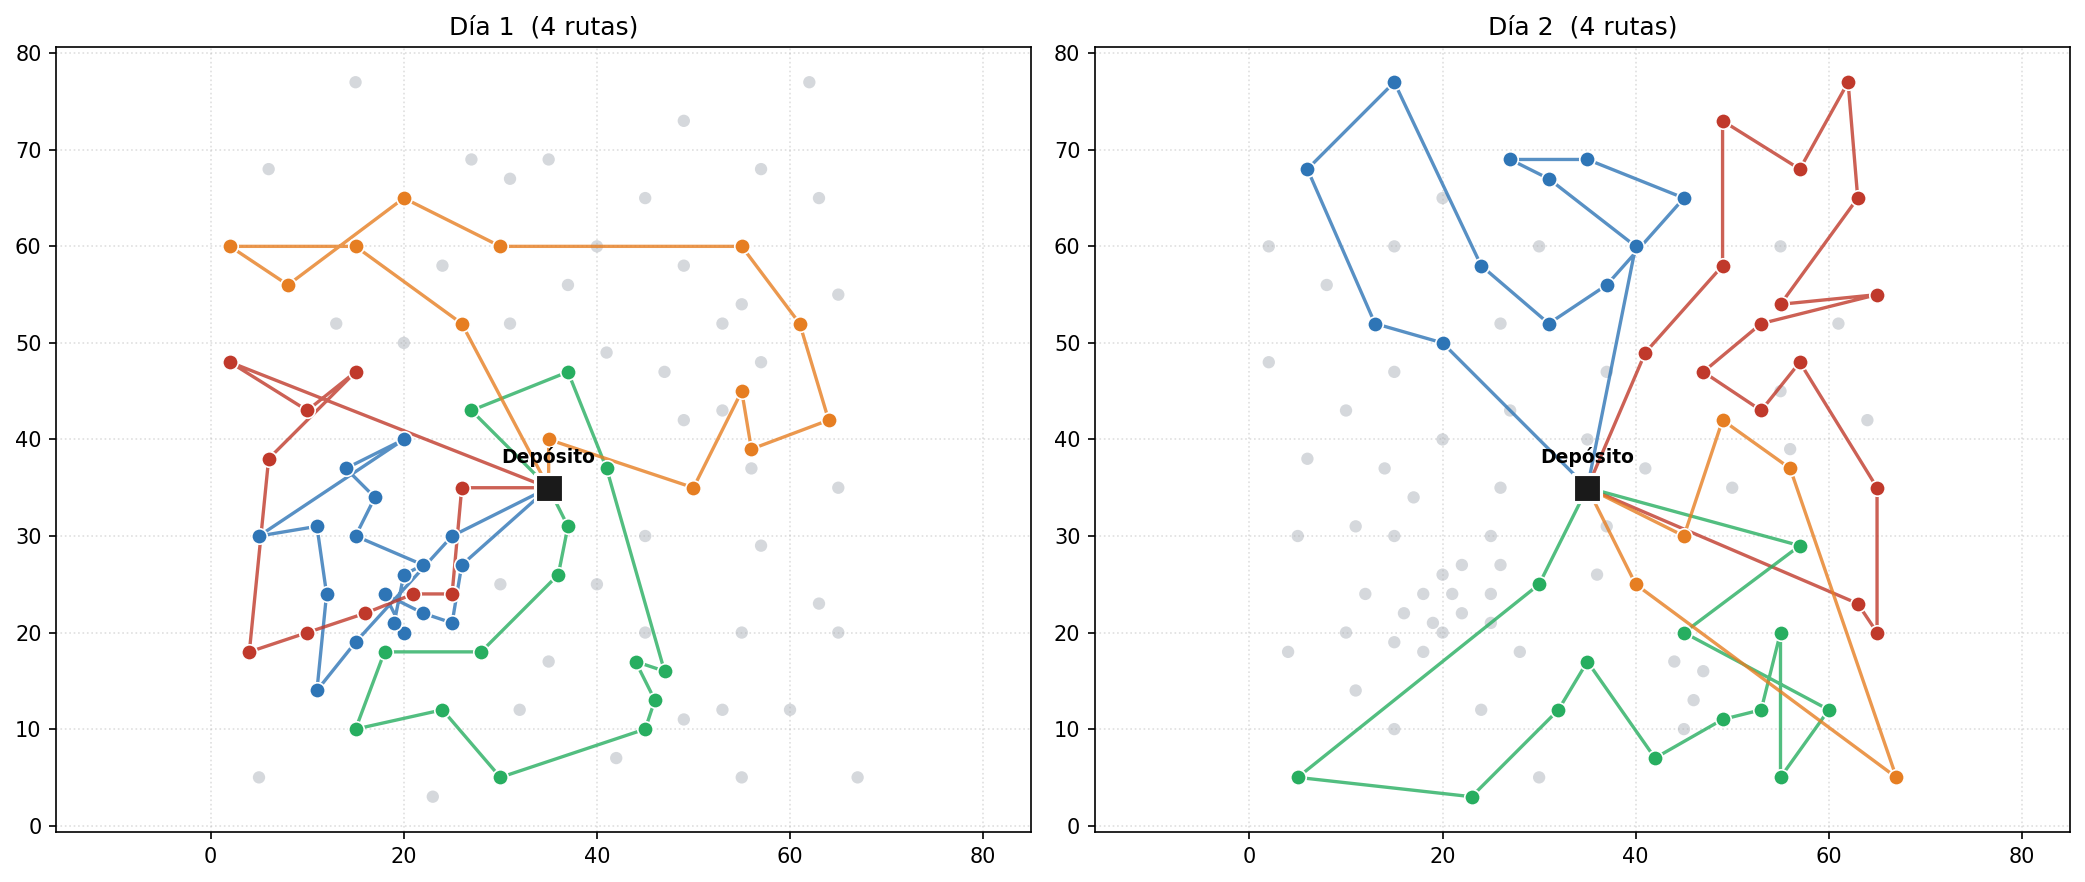
\includegraphics[width=\linewidth]{figures/rutas_p07_RL.png}
            \caption{Solución generada por el agente RL: Costo $1238.5$, factible.}
        \end{subfigure}

        \begin{subfigure}{0.95\textwidth}
            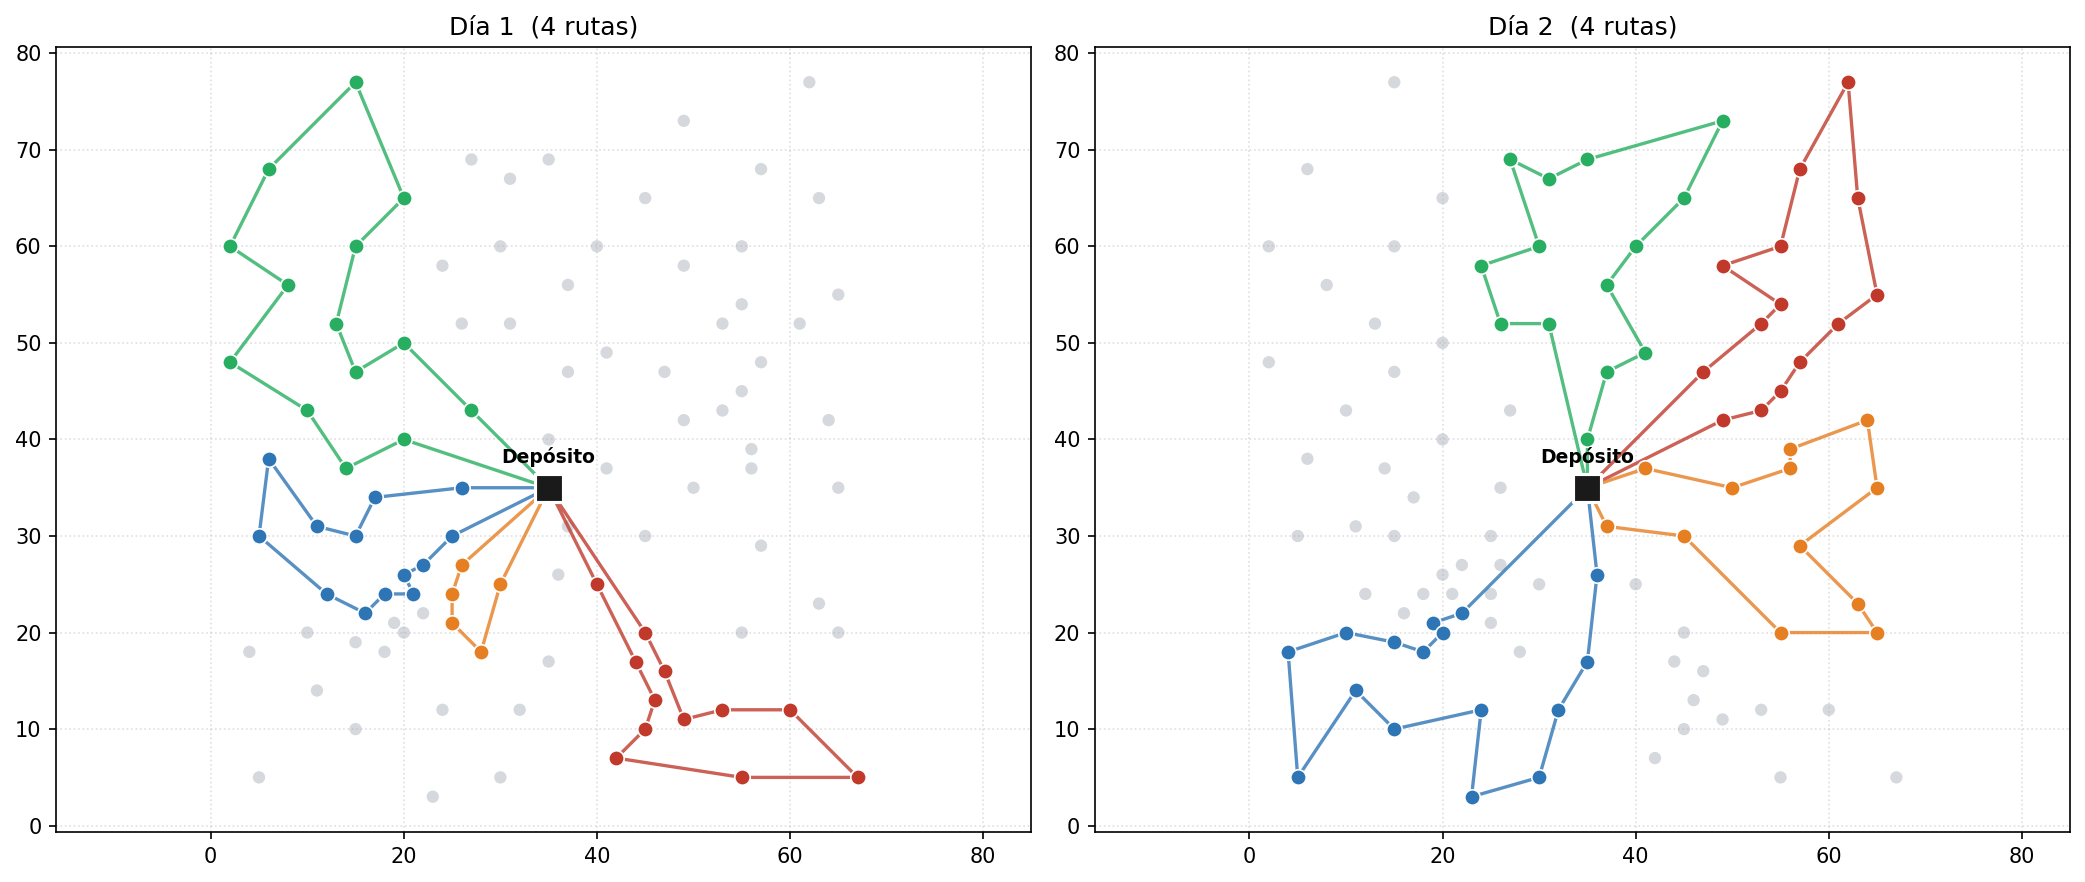
\includegraphics[width=\linewidth]{figures/rutas_p07_BKS.png}
            \caption{Mejor solución conocida BKS: Costo $826.1$.}
        \end{subfigure}
    \end{minipage}
    \caption{Rutas en la instancia $p07$.}
    \caption*{Fuente: Elaboración propia.}
    \label{fig:rutas-p07}
\end{figure}

\clearpage
\begin{figure}[H]
    \centering
    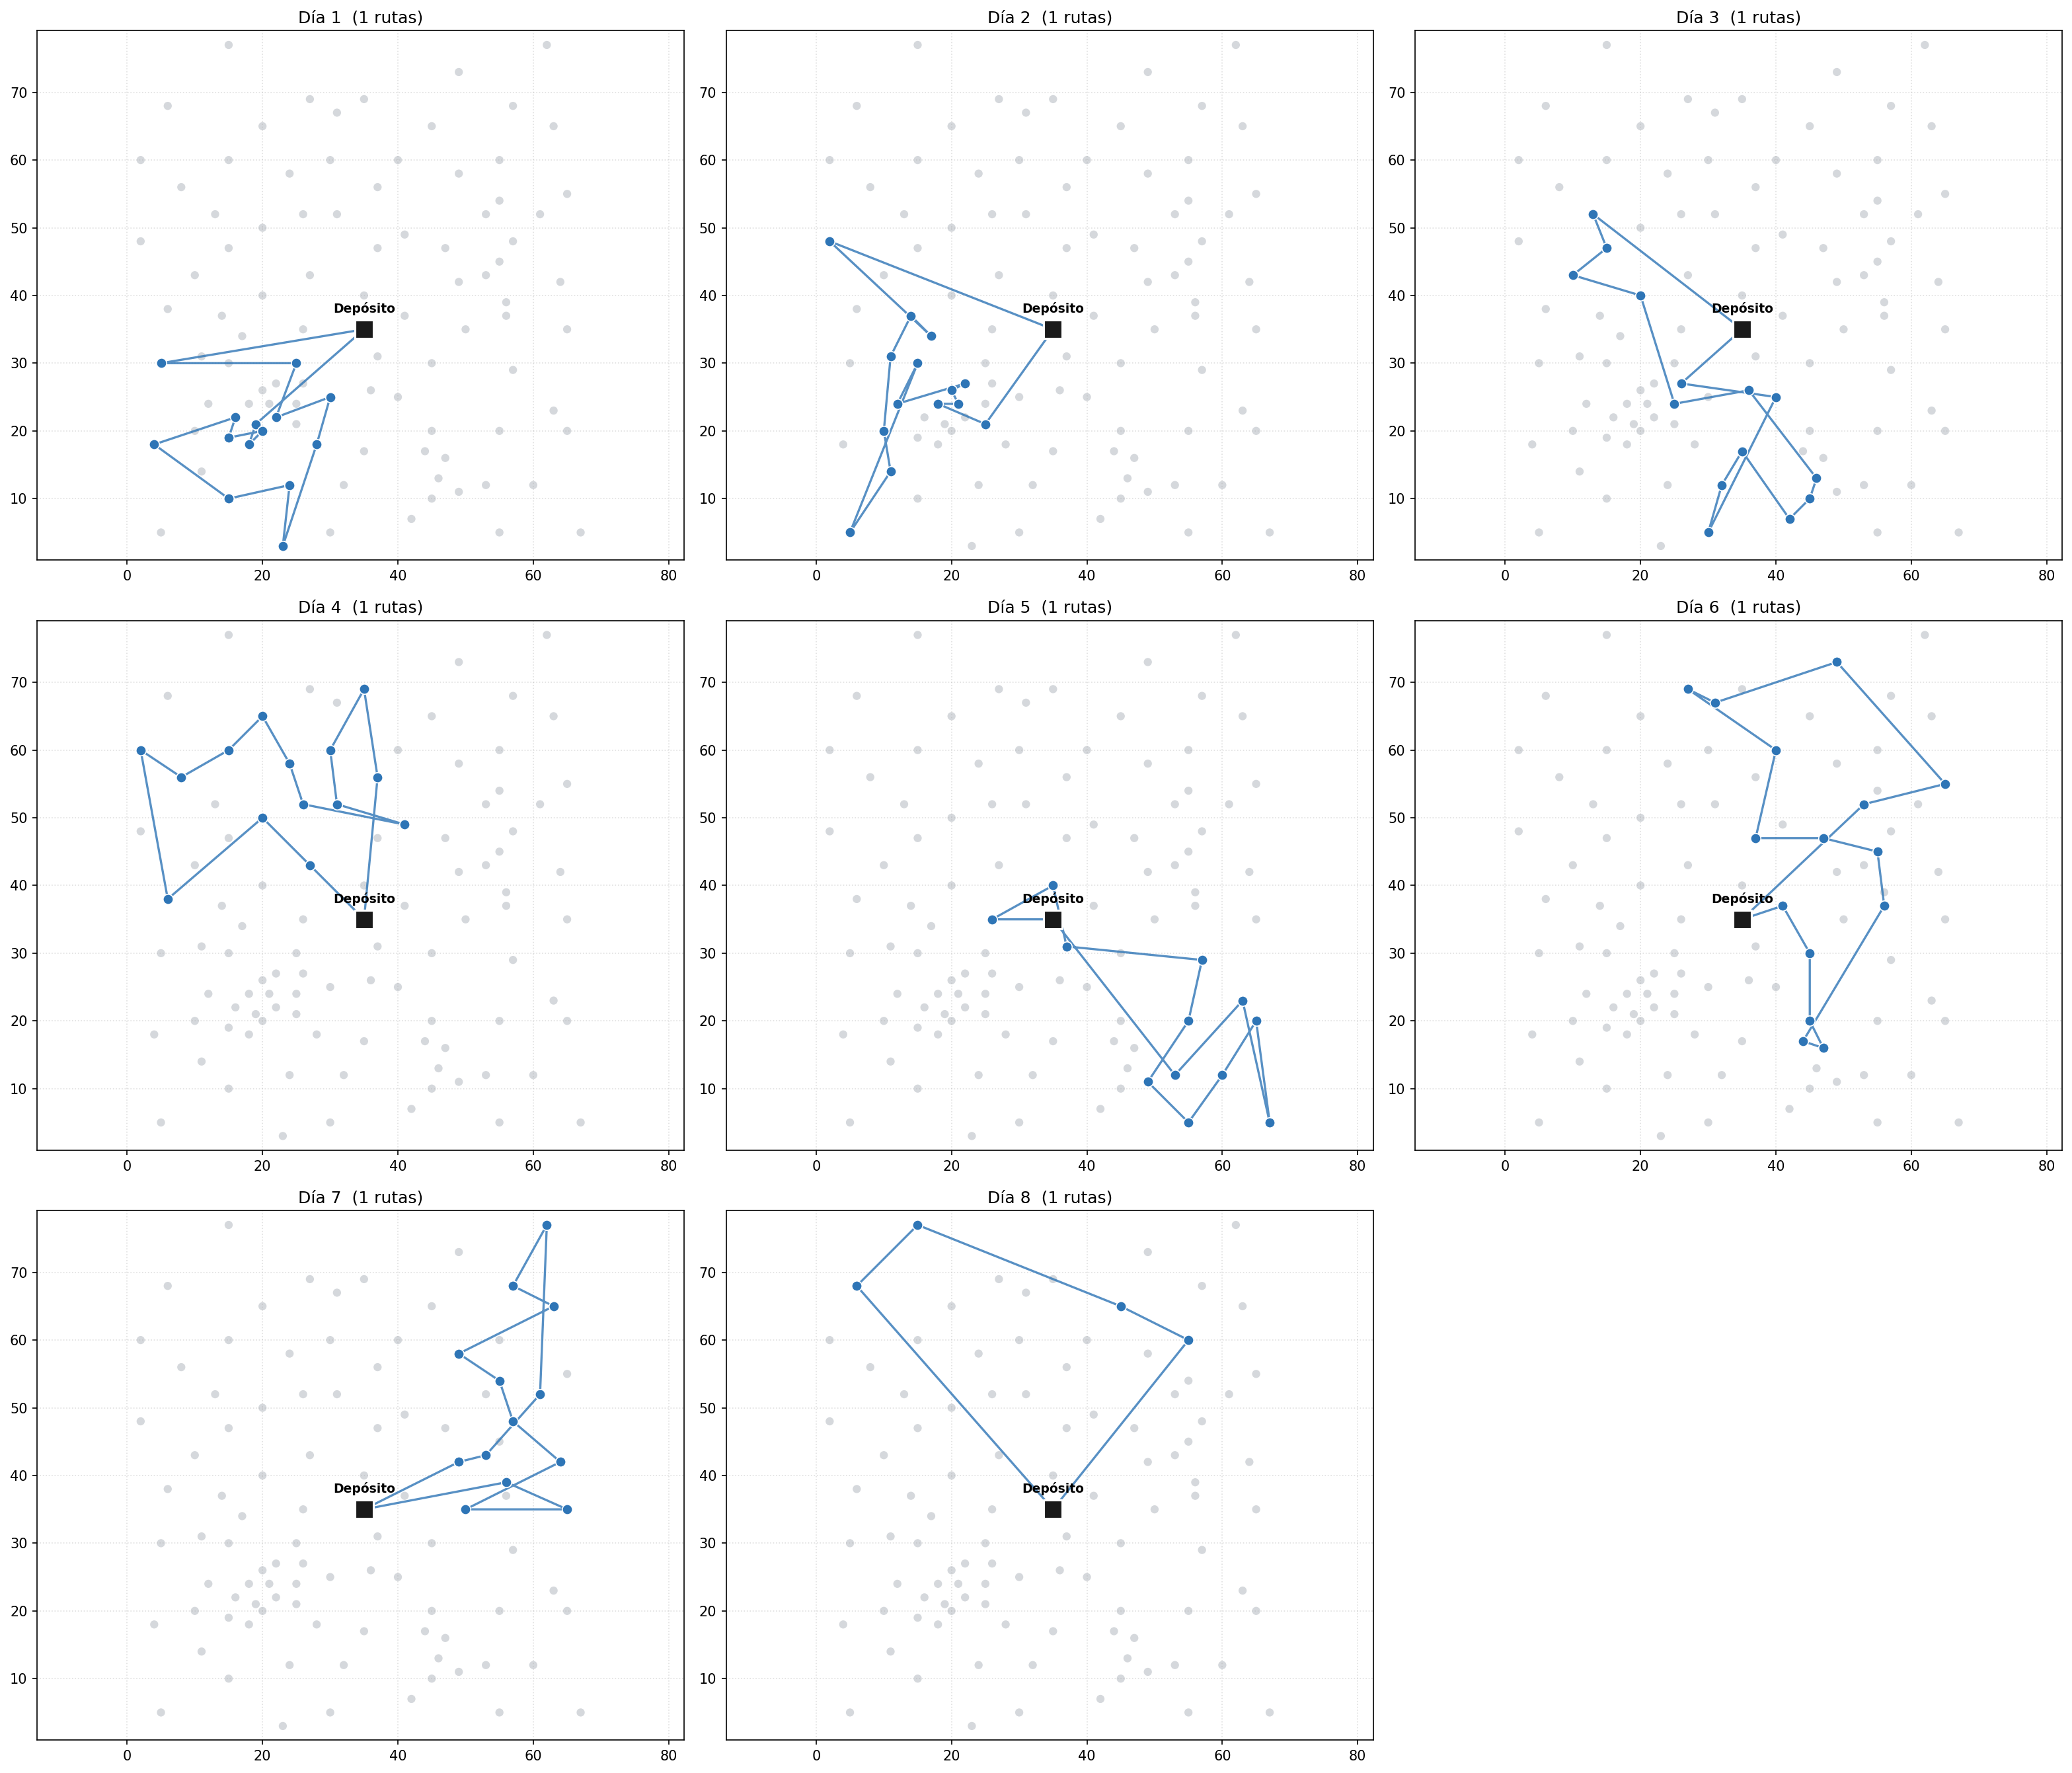
\includegraphics[
        width=\linewidth,
        height=0.80\textheight,
        keepaspectratio
    ]{figures/rutas_p09_RL.png}
    \caption{Rutas en la instancia $p09$ generadas por el agente RL: costo $1369{,}2$, factible.}
    \caption*{Fuente: Elaboración propia.}
    \label{fig:rutas-p09-rl}
\end{figure}

\clearpage
\begin{figure}[H]
    \centering
    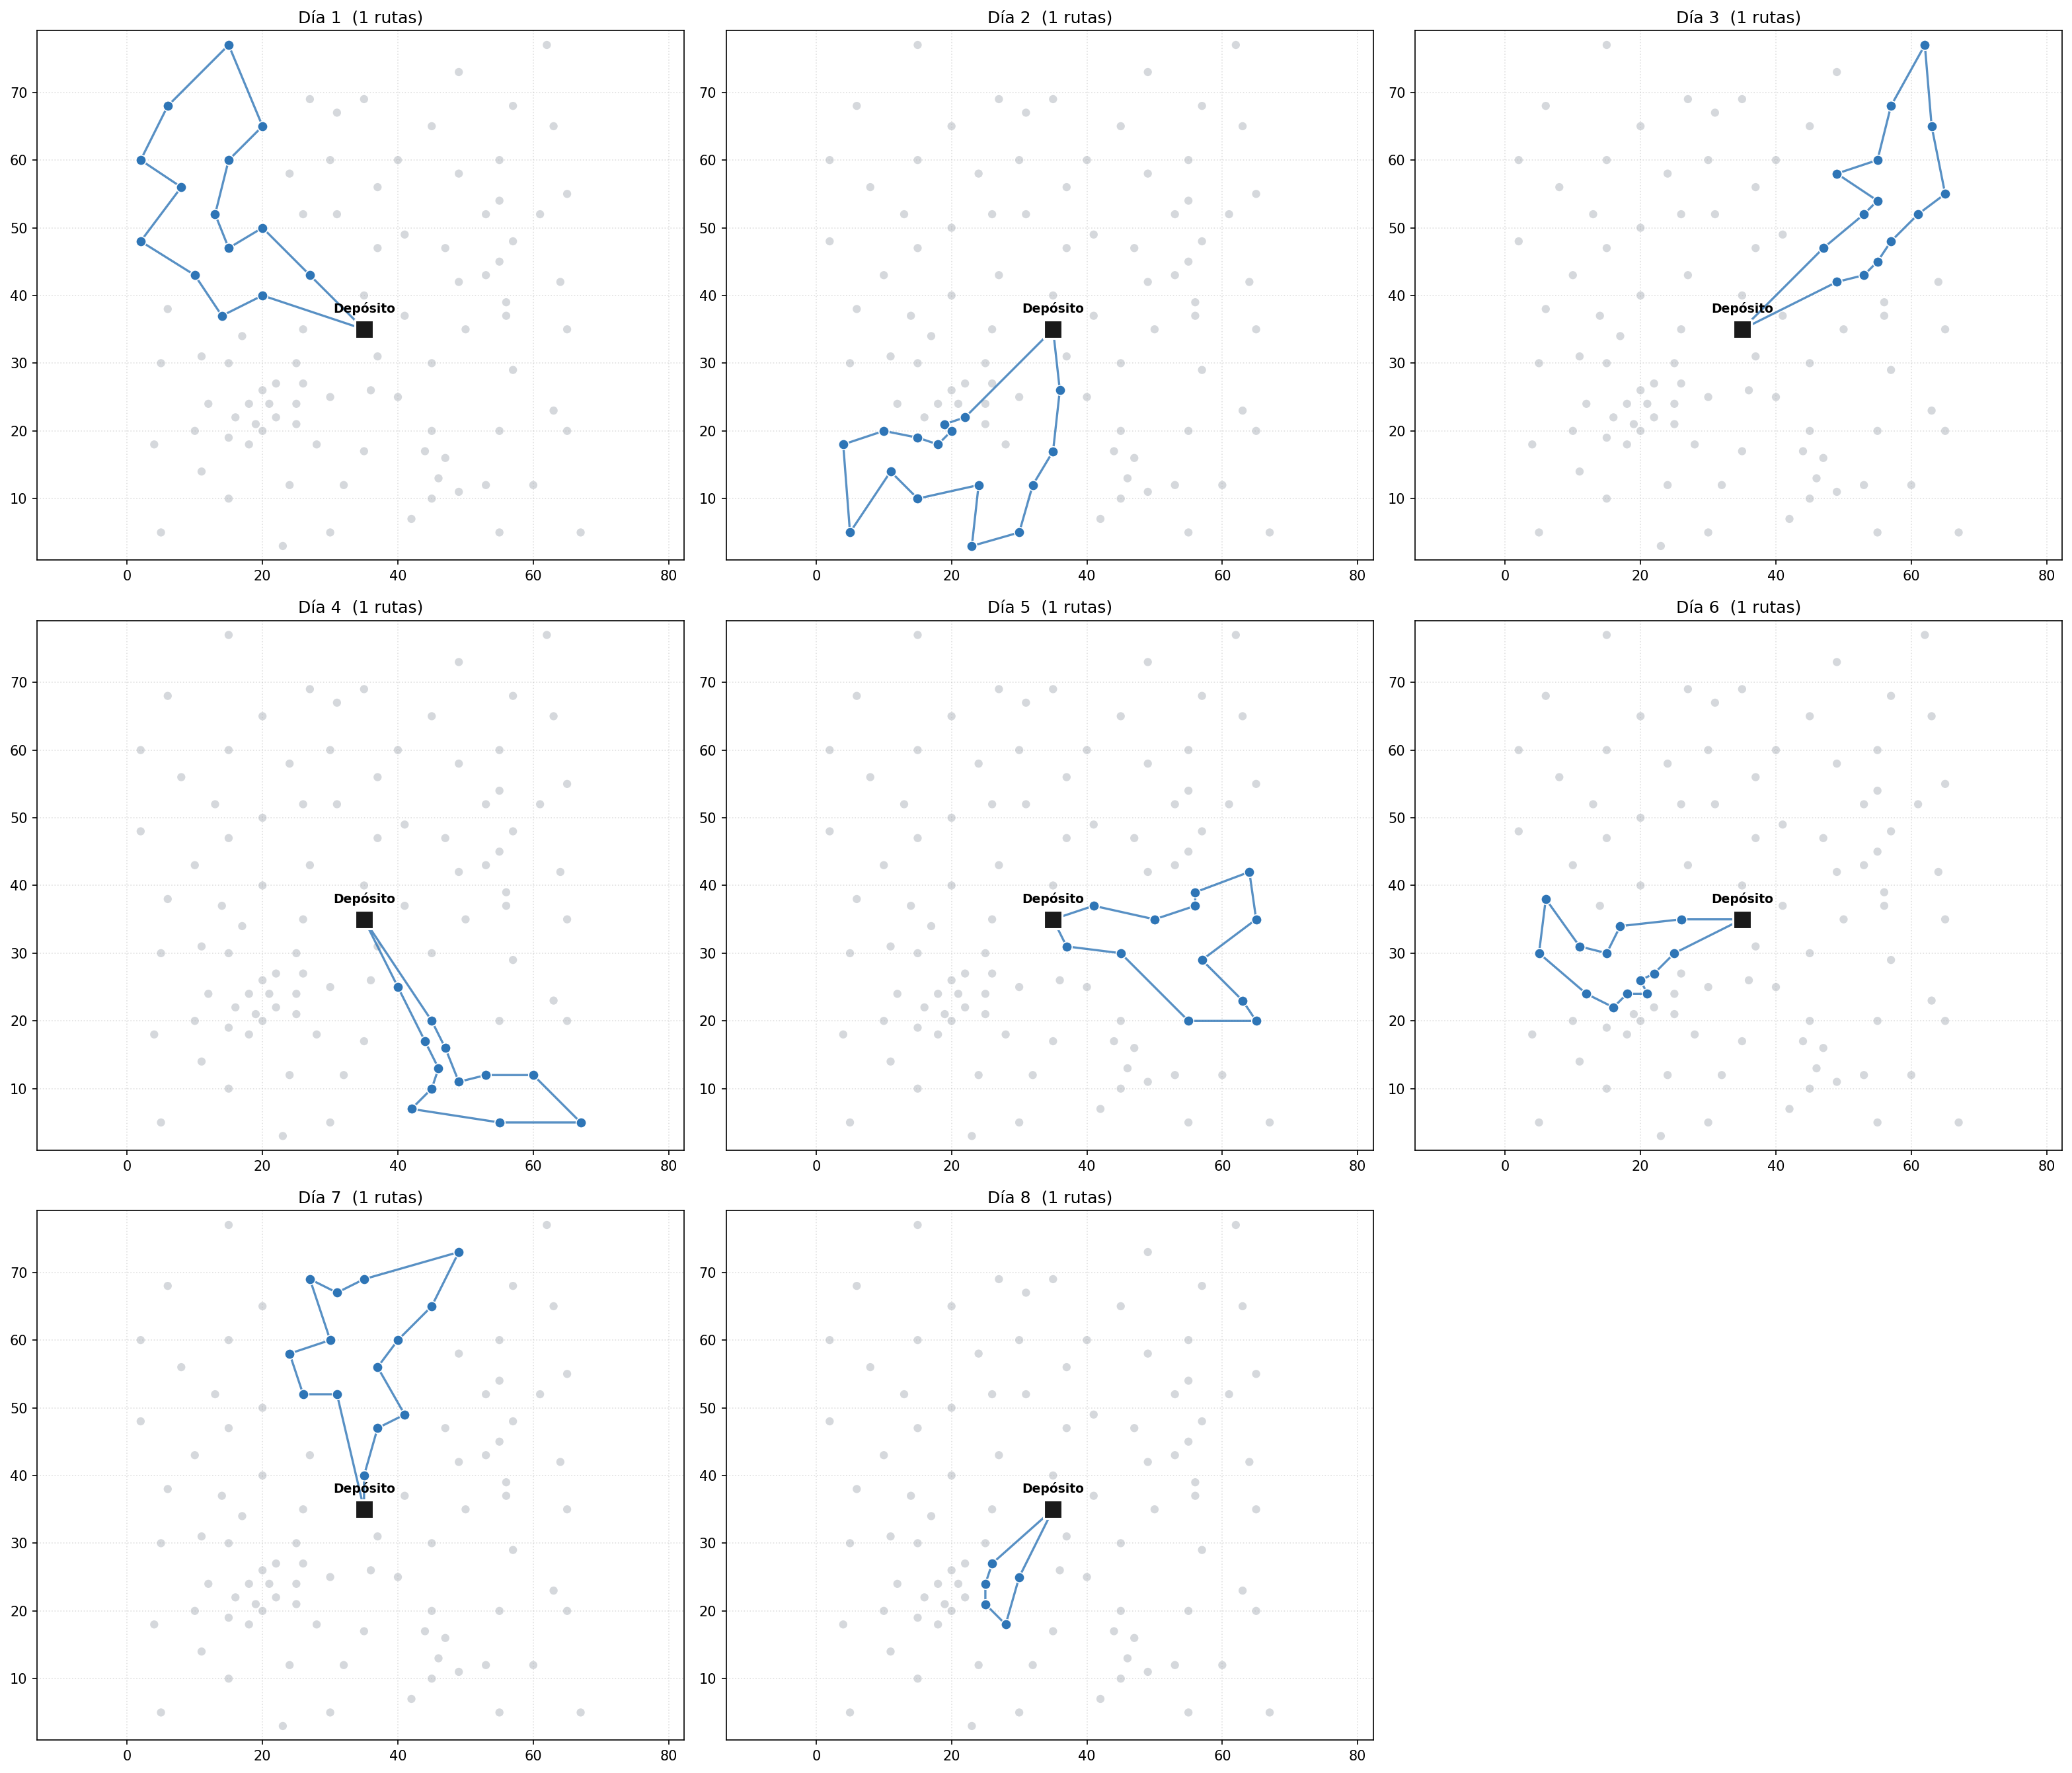
\includegraphics[
        width=\linewidth,
        height=0.80\textheight,
        keepaspectratio
    ]{figures/rutas_p09_BKS.png}
    \caption{Mejor solución conocida (BKS) para la instancia $p09$: costo $826{,}1$.}
    \caption*{Fuente: Elaboración propia.}
    \label{fig:rutas-p09-bks}
\end{figure}

\javi{Profe, arreglé los captions de p06 y p09: ahora cada parte (RL y BKS) tiene su propio caption y label, ninguna queda vacía. También cambié "mejores soluciones" por "soluciones representativas" para ser consistente con lo que aclaré en p01.}

%=============================================================%
\subsection{Identificación de los límites del método} \label{sec:limites}
%=============================================================%
Poner a prueba el modelo también implicó llevarlo hasta sus puntos de quiebre. Este proceso permitió identificar dos límites claros en el enfoque propuesto, los cuales se documentan y analizan a continuación.

%=============================================================%
\subsubsection{Límite combinatorio: familia B}
Al evaluar la instancia $p02$ (familia B, $50$ clientes, horizonte 5 días y 3 vehículos con multi-frecuencia), el patrón fue inequívoco: las cinco semillas entrenadas resultaron \emph{infactibles}, dejando clientes sin atender. La Tabla~\ref{tab:p02-detalle} muestra el detalle, incluyendo al VNS como referencia de un método que sí resuelve la instancia.

\begin{table}[H]
    \centering
    \caption{\label{tab:p02-detalle} Detalle multi-semilla sobre la instancia $p02$. Todas las semillas del agente resultan infactibles.}
    \caption*{Fuente: Elaboración propia.}
    \renewcommand{\arraystretch}{1.15}
    \setlength{\tabcolsep}{10pt}
    \begin{tabular}{@{}lccc@{}}
        \toprule
        \textbf{Semilla} & \textbf{Costo} & \textbf{Gap (\%)} & \textbf{Factibilidad} \\
        \midrule
        $0$ & $2038{,}28$ & $+54{,}1$ & infactible \\
        $1$ & $1955{,}38$ & $+47{,}8$ & infactible \\
        $2$ & $2068{,}85$ & $+56{,}4$ & infactible \\
        $3$ & $1961{,}22$ & $+48{,}3$ & infactible \\
        $4$ & $1514{,}45$ & $+14{,}5$ & infactible \\
        \midrule
        VNS (referencia) & $1587{,}71$ & $+20{,}0$ & factible \\
        \bottomrule
    \end{tabular}
\end{table}

A nivel técnico, es crucial aclarar que el costo y el gap reportados para estas semillas infactibles corresponden únicamente al costo de las rutas parciales que el agente logró construir, las cuales no cubren el total de la demanda. Por lo tanto, estos valores no se pueden comparar directamente con el gap de una solución completa como la de VNS. Por ejemplo, que la semilla $4$ tenga un gap aparentemente bajo ($+14{,}5\%$) no significa que sea una solución casi tan buena como VNS; es más barata simplemente porque omitió visitar a ciertos clientes. Para evitar interpretaciones erróneas, la columna de factibilidad siempre debe leerse en conjunto con el gap.

Tanto el VNS ($+20{,}0\%$, factible) como la heurística Greedy resuelven esta misma instancia sin dificultad, generando soluciones que cubren la totalidad de la demanda (sus resultados completos figuran en la Tabla~\ref{tab:consolidada}). Queda comprobado, entonces, que el problema sí admite una solución válida, y la falla es atribuible estrictamente a la naturaleza del agente y no a una imposibilidad estructural de la instancia.

El diagnóstico de la causa descarta una hipótesis inicial de saturación de capacidad: $p02$ tiene una saturación de $86\%$, menor que la de $p03$ ($97\%$), que sí se resuelve. La diferencia estructural relevante es la combinación de multi-frecuencia con múltiples vehículos por día: en $p02$ el agente debe coordinar simultáneamente qué clientes visitar, en qué días repetir las visitas y cómo distribuir la carga entre tres vehículos. Esta combinación de decisiones acopladas excede la capacidad del enfoque constructivo sin retroceso. \eli{¿Acá no hay BKS ó greedy?} \javi{Profe, dejé la tabla con RL + VNS para no saturarla, pero agregué en el texto que Greedy también resuelve p02 (sus datos completos, junto al BKS, están en la tabla consolidada). El punto clave es que ambos baselines la resuelven, así que la infactibilidad es del agente, no del problema.}

%=============================================================%
\subsubsection{Límite por saturación extrema: $p06$ semilla 4}
El segundo límite apareció en la instancia $p06$ (familia C, $75$ clientes, horizonte de 10 días, un vehículo y saturación $97\%$). En este caso, cuatro de las cinco semillas produjeron soluciones factibles con un desempeño muy consistente (gaps entre $+51{,}9\%$ y $+57{,}9\%$), pero la semilla $4$ resultó infactible. Es la única instancia del estudio donde la factibilidad cae del $100\%$ a un $4/5$.

A diferencia de lo que ocurre en $p02$, donde la falla es absoluta y sistemática, en $p06$ la infactibilidad es apenas ocasional. Esto indica un límite mucho menos rígido, provocado por la altísima exigencia de combinar una saturación extrema de capacidad con un horizonte de planificación muy largo (10 días). En estas condiciones de borde, el método mantiene su capacidad para encontrar rutas válidas en la gran mayoría de los intentos, pero pierde la garantía de factibilidad universal.

%=============================================================%
\subsection{Generalización} \label{subsec:generalizacion}
%=============================================================%
Como se definió en la Sección~\ref{sec:Metodosdeevaluacion}, el objetivo del eje de generalización es determinar si la política aprendida realmente captura principios de ruteo transferibles, o si simplemente se dedica a memorizar la secuencia de decisiones específica de la instancia con la que entrenó. Para responder a esta pregunta, se estructuraron dos experimentos utilizando las instancias de $50$ clientes ($p01$, $p02$, $p03$). Al compartir exactamente la misma dimensión de estado y de acciones, estas instancias permiten hacer una comparación controlada sin necesidad de recurrir a técnicas de relleno paramétrico.

Antes de interpretar los resultados, hay un detalle estructural clave a considerar: $p01$ (familia A) y $p03$ (familia C), pese a pertenecer a familias distintas, comparten exactamente la misma geometría de clientes. Tienen las mismas coordenadas, demandas y frecuencias de visita (todas iguales a 1). La única diferencia real entre ambas es el horizonte temporal y la cantidad de vehículos ($T{=}2, K{=}3$ en $p01$, frente a $T{=}5, K{=}1$ en $p03$). Esto convierte el cruce de modelos entre estas dos instancias en una prueba relevante, pues no se evalúa si el agente reconoce un mapa nuevo, sino si es capaz de adaptar su comportamiento a una configuración logística completamente distinta operando sobre el mismo espacio geográfico.

Es importante aclarar que los resultados de esta sección provienen de una única corrida por configuración, obtenida durante una fase exploratoria previa a la adopción del protocolo de cinco semillas del resto del capítulo. La razón es que estos experimentos de generalización tienen un carácter cualitativo: su objetivo no es cuantificar con precisión estadística el gap, sino inspeccionar el mecanismo de decisión del agente al enfrentarse a instancias no vistas. Como se detalla a continuación, las conclusiones se sustentan en el análisis directo de la secuencia de acciones paso a paso, y no en el valor agregado del costo, por lo que son robustas pese a provenir de una sola corrida. \eli{¿por qué?} \javi{Profe, aclaré el porqué: estos experimentos son cualitativos (miran el mecanismo de decisión paso a paso, no el número final), y por eso una corrida basta para la conclusión. La validación estadística con multi-semilla queda como trabajo futuro, lo menciono más abajo.}

Los hallazgos cualitativos que se describen a continuación son robustos, ya que se verificaron analizando directamente la secuencia de decisiones del agente paso a paso y no solo el costo agregado. No obstante, su validación estadística formal mediante múltiples semillas queda propuesta como trabajo futuro.

%=============================================================%
\subsubsection{Transferencia cero-shot}
La Tabla~\ref{tab:cero-shot} muestra qué ocurre al evaluar a los agentes especializados en $p01$ y en $p03$ directamente sobre las instancias que no vieron durante su entrenamiento, sin ningún tipo de reajuste o reentrenamiento previo. En palabras simples, esto corresponde a una evaluación cero-shot\footnote{En el ámbito del aprendizaje automático, la transferencia zero-shot o cero-shot consiste en someter a un modelo ya entrenado a un escenario o tarea completamente nueva, comprobando su capacidad de generalizar sin realizar ninguna actualización adicional en los parámetros de su red neuronal.}.

\begin{table}[H]
    \centering
    \caption{\label{tab:cero-shot} Transferencia cero-shot entre $p01$, $p02$ y $p03$. El agente evaluado sobre su propia instancia de entrenamiento se marca como referencia.}
    \caption*{Fuente: Elaboración propia.}
    \small
    \renewcommand{\arraystretch}{1.15}
    \setlength{\tabcolsep}{10pt}
    \begin{tabular}{@{}llcc@{}}
        \toprule
        \textbf{Agente} & \textbf{Evaluado en} & \textbf{Gap vs BKS} & \textbf{Factible} \\
        \midrule
        Especializado en $p01$ & $p01$ (referencia)     & $+17{,}7\%$ & sí \\
        Especializado en $p01$ & $p03$ (transferencia)  & $+17{,}7\%$ & sí \\
        Especializado en $p01$ & $p02$ (transferencia)  & $+25{,}6\%$ & NO \\
        \midrule
        Especializado en $p03$ & $p03$ (referencia)     & $+21{,}3\%$ & sí \\
        Especializado en $p03$ & $p01$ (transferencia)  & $+20{,}1\%$ & sí \\
        Especializado en $p03$ & $p02$ (transferencia)  & $+23{,}7\%$ & NO \\
        \bottomrule
    \end{tabular}
\end{table}

A simple vista, las transferencias cruzadas entre $p01$ y $p03$ parecen un éxito rotundo. En ambos casos la política mantiene la factibilidad y logra un gap casi idéntico al de su propia instancia de entrenamiento. Sin embargo, al revisar paso a paso las decisiones que tomó el agente (en lugar de mirar solo el costo final), se descubrió que detrás de estos números operan mecanismos completamente distintos, lo cual cambia drásticamente lo que se puede afirmar sobre la generalización del modelo.

Al llevar el agente especializado de $p01$ a $p03$, la secuencia completa de acciones que ejecutó resultó ser idéntica, paso a paso, a la que hizo en $p01$. Armó exactamente la misma partición de rutas y, por ende, obtuvo el mismo costo ($617{,}39$). Esto ocurre porque la estructura del entorno de simulación (el horizonte y el número de vehículos) limita el presupuesto máximo de rutas ($T \times K$), pero no impide al agente tomar sus decisiones habituales si no excede ese límite. La solución memorizada por el agente requería exactamente cinco rutas, lo cual cuadraba por mera casualidad con el presupuesto de ambas configuraciones (6 rutas posibles en $p01$, 5 rutas en $p03$). Por lo tanto, esta coincidencia no es evidencia de adaptación al contexto logístico. Es un caso de transferencia contingente, es decir, la política actuó de forma ciega ante el horizonte y los vehículos, y la solución resultó factible solo por \enquote{suerte} geométrica.

El caso inverso, el agente especializado en $p03$ evaluado en $p01$, es cualitativamente opuesto. Aquí, la secuencia de acciones diverge de su comportamiento original en $p03$ justo a partir del paso 22. Este es exactamente el instante en el que la variable de estado que codifica el vehículo activo comienza a ser distinta entre ambas instancias. $p01$ permite usar hasta tres vehículos por día, mientras que $p03$ obliga a cambiar de día tras usar uno. Al notar esta diferencia en el estado, el agente construye una configuración de rutas distinta, manteniendo la factibilidad y logrando incluso un mejor gap ($+20{,}1\%$ frente a $+21{,}3\%$). Esto sí constituye evidencia de adaptación genuina, es decir, la red neuronal leyó correctamente el contexto logístico del estado y modificó su estrategia sobre la marcha para ajustarse a las nuevas reglas.

Como era de esperarse, en ambos sentidos de transferencia la instancia $p02$ resultó infactible (gaps de $+25{,}6\%$ y $+23{,}7\%$). Esto refuerza el límite combinatorio documentado en la Sección~\ref{sec:limites}: ni siquiera un agente entrenado en otra instancia es capaz de sortear la barrera de coordinar multi-frecuencia con múltiples vehículos bajo esta arquitectura constructiva.

%=============================================================%
\subsubsection{Entrenamiento multi-instancia}
El segundo experimento consistió en entrenar a un solo agente sobre las tres instancias de $50$ clientes de forma simultánea. En la práctica, durante el entrenamiento el agente no se enfrenta siempre a la misma instancia, sino que estas se van rotando: en cada episodio se le presenta una de las tres ($p01$, $p02$ o $p03$), de modo que a lo largo del entrenamiento acumula experiencia sobre todas ellas. La hipótesis era que esta exposición a múltiples instancias produciría una política más robusta y generalizable que la de un agente especializado en una sola. La Tabla~\ref{tab:multi-instancia} muestra los resultados. \eli{esta parte no la entiendo.} \javi{Profe, reformulé la explicación: el entrenamiento multi-instancia significa que en cada episodio el agente entrena sobre una de las tres instancias (rotándolas), para que aprenda de todas a la vez. Antes decía "alternando cíclicamente" que era confuso.}

\begin{table}[H]
    \centering
    \caption{\label{tab:multi-instancia} Desempeño del agente entrenado bajo el esquema multi-instancia.}
    \caption*{Fuente: Elaboración propia.}
    \renewcommand{\arraystretch}{1.15}
    \setlength{\tabcolsep}{11pt}
    \begin{tabular}{@{}ccc@{}}
        \toprule
        \textbf{Instancia evaluada} & \textbf{Gap vs BKS} & \textbf{Factible} \\
        \midrule
        $p01$ & $+94{,}4\%$ & sí \\
        $p02$ & $+58{,}5\%$ & NO \\
        $p03$ & $+85{,}5\%$ & sí \\
        \bottomrule
    \end{tabular}
\end{table}

Los resultados contrastan drásticamente con los agentes especializados. En $p01$, el gap del agente multi-instancia se disparó a $+94{,}4\%$ (casi cinco veces peor que el $+17{,}7\%$ original). En $p03$, la caída es igual de severa ($+85{,}5\%$ frente a $+21{,}3\%$). La razón detrás de esta degradación radica en la heterogeneidad estructural del entrenamiento. Mientras $p01$ exige optimizar dos días con tres vehículos, $p03$ impone cinco días con un solo vehículo. Al obligar a una única red a asimilar dinámicas temporales tan dispares, la política termina diluyendo su capacidad de representación. En lugar de volverse experta en un problema, alcanza un desempeño mediocre en todos. Esto se confirma al revisar la tasa de episodios factibles durante su entrenamiento: el agente multi-instancia se estancó entre un $56\%$ y un $60\%$, muy por debajo del prácticamente $100\%$ que alcanzan rápidamente los agentes especialistas.

%=============================================================%
\subsubsection{Síntesis del eje de generalización}
La transferencia contingente, la adaptación genuina y el colapso del entrenamiento multi-instancia entregan una respuesta llena de matices. El agente efectivamente es capaz de generalizar su comportamiento a configuraciones logísticas nuevas cuando logra percibir la diferencia en su vector de estado (caso $p03 \rightarrow p01$). Sin embargo, también demostró que puede arrojar resultados aparentemente exitosos por motivos ajenos al aprendizaje (caso $p01 \rightarrow p03$), lo que subraya lo importante que es inspeccionar siempre los mecanismos de la red neuronal y no confiarse únicamente en un buen número en el costo final.

Por otro lado, obligar al agente a generalizar mediante un entrenamiento multi-instancia sacrificó fuertemente la calidad de sus soluciones, evidenciando una fuerte tensión entre especialización y generalización, algo muy característico del Aprendizaje por Refuerzo en optimización combinatoria~\cite{nazari2018reinforcementlearningsolvingvehicle}.

%=============================================================%
\subsection{Comparación global con los baselines} \label{sec:comparacion-global}
%=============================================================%
La Tabla~\ref{tab:consolidada} consolida los resultados de los tres métodos sobre las nueve instancias evaluadas, y la Figura~\ref{fig:barras-comparativo} permite visualizarlos de forma directa. En este gráfico y en la tabla, las instancias $p05$ y $p08$ figuran como \enquote{no evaluado} para el agente RL. Esta decisión se sustenta en dos motivos técnicos y prácticos. Primero, la evaluación previa de $p02$ ($50$ clientes, familia B) resultó infactible en sus cinco semillas, evidenciando un claro límite combinatorio. Como $p05$ y $p08$ comparten exactamente las mismas características estructurales (horizonte medio, múltiples vehículos por día y patrones multi-frecuencia coordinados), el resultado esperable sería análogo o peor. Segundo, el entrenamiento con la red ampliada ($[512, 512]$, $500\,000$ pasos) exige cerca de dos horas de cómputo por instancia para completar las cinco semillas. Por lo tanto, se priorizaron esos recursos para escalar las familias donde el método sí alcanza factibilidad ($p04$, $p06$, $p07$, $p09$) y entender mejor su verdadero rango de aplicabilidad. Por su parte, los métodos Greedy y VNS sí se ejecutaron en toda la familia B, confirmando que estas instancias admiten soluciones factibles mediante heurísticas clásicas.

\begin{table}[H]
    \centering
    \caption{\label{tab:consolidada} Resultados consolidados sobre las nueve instancias del conjunto NEO evaluadas. Gap respecto a la mejor solución conocida, en porcentaje. El agente RL se reporta como media sobre semillas factibles.}
    \caption*{Fuente: Elaboración propia.}
    \small
    \renewcommand{\arraystretch}{1.15}
    \setlength{\tabcolsep}{7pt}
    \begin{tabular}{@{}cccccc@{}}
        \toprule
        \textbf{Familia} & \textbf{Instancia} & \textbf{Greedy} & \textbf{VNS} & \textbf{RL} & \textbf{Factib. RL} \\
        \midrule
        \multirow{3}{*}{A} & $p01$ &  $+70{,}2\%$ &  $+31{,}7\%$ & $+19{,}7\%$  & $5/5$ \\
                           & $p04$ & $+212{,}8\%$ &  $+23{,}1\%$ & $+53{,}9\%$  & $5/5$ \\
                           & $p07$ &  $+75{,}1\%$ &  $+27{,}3\%$ & $+57{,}4\%$  & $5/5$ \\
        \midrule
        \multirow{3}{*}{B} & $p02$ &  $+44{,}0\%$ &  $+20{,}0\%$ & infactible   & $0/5$ \\
                           & $p05$ &  $+53{,}9\%$ &  $+17{,}0\%$ & no evaluado  & --- \\
                           & $p08$ &  $+52{,}9\%$ &  $+18{,}3\%$ & no evaluado  & --- \\
        \midrule
        \multirow{3}{*}{C} & $p03$ & $+100{,}2\%$ &  $+83{,}8\%$ & $+28{,}0\%$  & $5/5$ \\
                           & $p06$ & $+118{,}5\%$ & $+104{,}7\%$ & $+55{,}7\%$  & $4/5$ \\
                           & $p09$ & $+156{,}9\%$ & $+128{,}5\%$ & $+66{,}7\%$  & $5/5$ \\
        \bottomrule
    \end{tabular}
\end{table}

\begin{figure}[H]
    \centering
    \begin{tikzpicture}
        \begin{axis}[
            width=10.8cm,
            height=7cm,
            ybar=2pt,
            bar width=6pt,
            ylabel={Gap respecto al BKS (\%)},
            symbolic x coords={p01,p02,p03,p04,p05,p06,p07,p08,p09},
            xtick=data,
            ymin=0,
            ymax=230,
            ytick={0,50,100,150,200},
            grid=major,
            xmajorgrids=true,
            ymajorgrids=true,
            grid style={line width=0.3pt, draw=gray!30},
            axis line style={black!70},
            tick style={black!70},
            tick label style={font=\small},
            label style={font=\small},
            enlarge x limits=0.10,
            legend style={
                font=\small,
                draw=black!40,
                fill=white,
                rounded corners=2pt,
                at={(1.04,0.5)},
                anchor=west
            },
            legend cell align=left,
            clip=false
        ]
            \addplot[draw=greedyLine, fill=greedyFill] coordinates {
                (p01,70.2) (p02,44.0) (p03,100.2) (p04,212.8)
                (p05,53.9) (p06,118.5) (p07,75.1) (p08,52.9) (p09,156.9)
            };
            \addlegendentry{Greedy}

            \addplot[draw=vnsLine, fill=vnsFill] coordinates {
                (p01,31.7) (p02,20.0) (p03,83.8) (p04,23.1)
                (p05,17.0) (p06,104.7) (p07,27.3) (p08,18.3) (p09,128.5)
            };
            \addlegendentry{VNS}

            \addplot[draw=rlLine, fill=rlFill] coordinates {
                (p01,19.7) (p03,28.0) (p04,53.9)
                (p06,55.7) (p07,57.4) (p09,66.7)
            };
            \addlegendentry{RL}
        \end{axis}
    \end{tikzpicture}
    \caption{Comparación del gap respecto al BKS de los tres métodos sobre las instancias evaluadas. Las instancias $p02$, $p05$ y $p08$ (familia B) no presentan barra de RL por resultar infactibles o no evaluadas.}
    \caption*{Fuente: Elaboración propia.}
    \label{fig:barras-comparativo}
\end{figure}

El análisis global de estos datos revela tres escenarios operativos muy claros:

\begin{itemize}
    \item En $50$ clientes (familias A y C), el agente RL supera a VNS: logra $+19{,}7\%$ frente a $+31{,}7\%$ en $p01$, y un aplastante $+28{,}0\%$ frente a $+83{,}8\%$ en $p03$.

    \item En $75$ y $100$ clientes (familias A y C), VNS supera al RL: por ejemplo, logra un $+23{,}1\%$ frente al $+53{,}9\%$ del agente en $p04$. Esto ocurre porque el refinamiento local del VNS rinde mucho más al crecer la instancia, mientras que el enfoque puramente constructivo del RL pierde calidad geométrica.

    \item En la familia B, VNS logra resolver el problema mientras el RL no alcanza la factibilidad, un límite combinatorio que se mantiene incluso al intentar aplicar transferencia de aprendizaje desde otras instancias.
\end{itemize}

Sin embargo, este panorama cambia drásticamente al analizar los tiempos de inferencia, donde el agente RL demuestra una superioridad absoluta. La Tabla~\ref{tab:tiempos} y la Figura~\ref{fig:tiempos} resumen el tiempo de ejecución requerido por cada método en las distintas instancias.

\begin{table}[H]
    \centering
    \caption{\label{tab:tiempos} Tiempos de inferencia/ejecución de los tres métodos por instancia.}
    \caption*{Fuente: Elaboración propia.}
    \renewcommand{\arraystretch}{1.15}
    \setlength{\tabcolsep}{10pt}
    \begin{tabular}{@{}cccc@{}}
        \toprule
        \textbf{Instancia} & \textbf{Greedy} & \textbf{VNS} & \textbf{RL (inferencia)} \\
        \midrule
        $p01$ & $0{,}007$ s & $3{,}368$ s & $\sim 0{,}04$ s \\
        $p02$ & $0{,}010$ s & $5{,}110$ s & $\sim 0{,}04$ s \\
        $p03$ & $0{,}006$ s & $0{,}239$ s & $\sim 0{,}04$ s \\
        $p04$ & $0{,}019$ s & $5{,}346$ s & $\sim 0{,}06$ s \\
        $p05$ & $0{,}026$ s & $11{,}842$ s & --- \\
        $p06$ & $0{,}012$ s & $0{,}330$ s & $\sim 0{,}06$ s \\
        $p07$ & $0{,}036$ s & $21{,}897$ s & $\sim 0{,}08$ s \\
        $p08$ & $0{,}077$ s & $38{,}740$ s & --- \\
        $p09$ & $0{,}023$ s & $0{,}840$ s & $\sim 0{,}08$ s \\
        \bottomrule
    \end{tabular}
\end{table}

\begin{figure}[H]
    \centering
    \begin{tikzpicture}
        \begin{semilogyaxis}[
            width=10.8cm,
            height=7cm,
            ylabel={Tiempo (segundos, escala logarítmica)},
            symbolic x coords={p01,p02,p03,p04,p05,p06,p07,p08,p09},
            xtick=data,
            ymin=0.001,
            ymax=100,
            ytick={0.001,0.01,0.1,1,10,100},
            grid=major,
            xmajorgrids=true,
            ymajorgrids=true,
            grid style={line width=0.3pt, draw=gray!30},
            axis line style={black!70},
            tick style={black!70},
            tick label style={font=\small},
            label style={font=\small},
            enlarge x limits=0.10,
            legend style={
                font=\small,
                draw=black!40,
                fill=white,
                rounded corners=2pt,
                at={(1.04,0.5)},
                anchor=west
            },
            legend cell align=left,
            clip=false
        ]
            \addplot[color=greedyLine, thick, mark=square*, mark size=2.4pt]
            coordinates {
                (p01,0.007) (p02,0.010) (p03,0.006) (p04,0.019)
                (p05,0.026) (p06,0.012) (p07,0.036) (p08,0.077) (p09,0.023)
            };
            \addlegendentry{Greedy}

            \addplot[color=vnsLine, thick, mark=triangle*, mark size=2.8pt]
            coordinates {
                (p01,3.368) (p02,5.110) (p03,0.239) (p04,5.346)
                (p05,11.842) (p06,0.330) (p07,21.897) (p08,38.740) (p09,0.840)
            };
            \addlegendentry{VNS}

            \addplot[color=rlLine, thick, mark=*, mark size=2.8pt]
            coordinates {
                (p01,0.04) (p02,0.04) (p03,0.04) (p04,0.06)
                (p06,0.06) (p07,0.08) (p09,0.08)
            };
            \addlegendentry{RL}
        \end{semilogyaxis}
    \end{tikzpicture}
    \caption{Tiempos de inferencia de los tres métodos por instancia, en escala logarítmica.}
    \caption*{Fuente: Elaboración propia.}
    \label{fig:tiempos}
\end{figure}

Queda en evidencia que el agente entrega su solución entre uno y dos órdenes de magnitud más rápido que VNS. En instancias grandes (como $p07$), donde el VNS requiere decenas de segundos para terminar su proceso, el agente entrenado responde en menos de una décima de segundo. Esta ventaja resulta de suma importancia para escenarios operativos reales, donde el costo logístico de la ruta debe equilibrarse con la necesidad de obtener tiempos de respuesta casi inmediatos.

Los tiempos reportados hasta ahora corresponden a la fase de inferencia; el entrenamiento del agente constituye una inversión de cómputo previa y única por instancia. La configuración base ($300\,000$ pasos, red $[256,256]$) requirió aproximadamente $9$ minutos por semilla en CPU estándar, sumando cerca de $45$ minutos por instancia bajo el protocolo multi-semilla. La configuración escalada ($500\,000$ pasos, red $[512,512]$) requirió aproximadamente $20$ minutos por semilla, es decir, cerca de $100$ minutos por instancia. En agregado, los siete análisis multi-semilla completos totalizaron alrededor de $7$ horas de cómputo. Es relevante destacar que este costo se paga una única vez: una vez entrenado, el agente resuelve nuevas ejecuciones de la misma instancia en fracciones de segundo, lo que sostiene su ventaja operativa frente a VNS en escenarios de uso repetido o de respuesta rápida. Cabe subrayar, además, que todo el entrenamiento se ejecutó sin aceleración por GPU, lo que refuerza la accesibilidad del método en infraestructura de cómputo convencional. 

\eli{Hablar de tiempos de entrenamiento.} 
\javi{Profe, agregué el párrafo de tiempos de entrenamiento con datos reales: ~9 min/semilla en config base, ~20 min/semilla en escalada, ~7 horas agregadas, todo en CPU sin GPU. El punto clave es que es un costo único (se entrena una vez y luego infiere instantáneo), a diferencia de VNS que repite su búsqueda cada vez.}

%=============================================================%
\subsection{Síntesis de la validación} \label{sec:sintesis-validacion}
%=============================================================%
La Tabla~\ref{tab:sintesis-familias} resume los hallazgos agrupados por familia estructural, incorporando además las observaciones del eje de generalización.

\begin{table}[H]
    \centering
    \caption{\label{tab:sintesis-familias} Síntesis de los resultados por familia estructural.}
    \caption*{Fuente: Elaboración propia.}
    \small
    \renewcommand{\arraystretch}{1.18}
    \setlength{\tabcolsep}{7pt}
    \begin{tabularx}{\textwidth}{@{}>{\centering\arraybackslash}p{1.5cm}XX@{}}
        \toprule
        \textbf{Familia} & \textbf{Calidad y robustez} & \textbf{Generalización} \\
        \midrule
        A & Factibilidad universal ($15/15$ corridas). Supera a VNS en $50$ clientes ($p01$); VNS supera al RL en $75$ y $100$ clientes ($p04$, $p07$). Degradación predecible al escalar. & Transferencia hacia $p03$ (familia~C, misma geometría): contingente en un sentido, genuina en el otro. \\
        \midrule
        B & Infactibilidad sistemática en $p02$ ($0/5$ corridas factibles). Límite combinatorio identificado: el enfoque constructivo no coordina visitas multi-frecuencia entre múltiples vehículos. & Infactibilidad persiste bajo transferencia desde $p01$ y $p03$; el límite combinatorio es robusto a la estrategia de entrenamiento. \\
        \midrule
        C & Factibilidad alta ($14/15$ corridas). Supera a VNS en todas las escalas evaluadas con factibilidad ($p03$, $p06$, $p09$). Una infactibilidad ocasional en $p06$ semilla $4$. & Transferencia hacia $p01$ (familia~A, misma geometría): adaptación genuina verificada a nivel de secuencia de decisiones. \\
        \bottomrule
    \end{tabularx}
\end{table}

A partir de toda la evidencia recolectada a lo largo de este capítulo, se concluyen seis afirmaciones sobre el desempeño del modelo:

\begin{enumerate}
    \item \textbf{Superioridad inicial:} El agente supera al VNS en instancias de $50$ clientes (familias A y C), entregando mejores rutas en tiempos de inferencia que resultan ser entre uno y dos órdenes de magnitud menores.

    \item \textbf{Escalamiento robusto:} El método logra escalar a problemas de $75$ y $100$ clientes manteniendo una factibilidad casi universal ($29/30$ corridas factibles). Sin embargo, tal como evidencian los gráficos de rutas, pierde calidad geométrica relativa frente a la heurística de mejora local al aumentar la densidad de clientes.

    \item \textbf{Estabilidad operativa:} El comportamiento de la red neuronal es reproducible y predecible. La desviación estándar del gap entre las distintas semillas se mantuvo siempre acotada entre un $\pm 5\%$ y un $\pm 7\%$ en todas las configuraciones evaluadas.

    \item \textbf{Límite combinatorio transparente:} Se identificó una barrera técnica clara en la familia B. El agente puramente constructivo no logra coordinar decisiones de multi-frecuencia entre múltiples vehículos de forma simultánea, fallando en alcanzar la factibilidad en escenarios que el VNS resuelve con facilidad.

    \item \textbf{Velocidad de respuesta:} El agente ofrece una ventaja operativa sustancial en el tiempo de inferencia. En las instancias más grandes resuelve todo el ruteo en fracciones de segundo, posicionándolo como una alternativa altamente competitiva para entornos reales que exigen respuestas rápidas.

    \item \textbf{Generalización con matices:} Se comprobó que el agente no solo memoriza, sino que puede adaptar genuinamente su comportamiento a un nuevo contexto logístico si el vector de estado lo refleja ($p03 \rightarrow p01$). No obstante, también se descubrió que puede generar resultados \enquote{exitosos} por pura coincidencia geométrica ciega ($p01 \rightarrow p03$). Además, se confirmó que el entrenamiento multi-instancia genera una fuerte tensión con la especialización, degradando fuertemente el desempeño global del agente.
\end{enumerate}

Con esta validación, se demostró empíricamente que el enfoque basado en Aprendizaje por Refuerzo es competitivo, estable y extremadamente veloz dentro de su régimen de aplicabilidad. Al mismo tiempo, se delimitó con total transparencia las fronteras donde el modelo falla y requiere apoyo. Estos hallazgos preparan el terreno para el siguiente Capítulo, donde se plantearán las conclusiones finales de la memoria y se propondrán las líneas de trabajo futuro.